\documentclass[12pt]{article}
\usepackage{amsmath}
\usepackage[utf8]{inputenc}
\usepackage[authoryear, round]{natbib}
\usepackage{graphicx}
\usepackage[left=4cm,right=2cm,outer=2cm,bottom=2cm,top=2cm]{geometry}
\usepackage{mathrsfs}
\usepackage{subfig}
\usepackage[onehalfspacing]{setspace}
\usepackage{hyperref}
\usepackage{scrpage2}

\ifoot[]{}
\cfoot[]{}
\ofoot[\pagemark]{\pagemark}

\pagestyle{scrplain}

\linespread{1.5}
\let\oldfootnotesize\footnotesize
\renewcommand*{\footnotesize}{\oldfootnotesize\fontsize{10pt}{0}\selectfont}
\newcommand{\HRule}{\rule{\linewidth}{0.5mm}}


\pagenumbering{roman}



\title{\textbf{Predicting Economic Time-Series using Dynamic Factor Models under Structural Breaks}}
\author{Johannes Degn}
\date{07.07.2014}
\begin{document}

\titlepage
\thispagestyle{empty}
\setcounter{page}{0}

\begin{titlepage}
\begin{center}
	University of Konstanz

	\vspace{2cm}
	\HRule
	\vspace{1cm}
	\large{Predicting Economic Time-Series using Dynamic Factor Models under Structural Breaks}
	\vspace{1cm}
	\HRule
    \vspace{1cm}
    
	\begin{minipage}{0.4\textwidth}
		\begin{flushleft}
			\emph{Author:} \\
			Johannes Degn
		\end{flushleft}
	\end{minipage}
	\begin{minipage}{0.4\textwidth}
		\begin{flushright}
			\emph{Supervisor:} \\
			Ralf Brüggemann
		\end{flushright}
	\end{minipage}
    \vspace{8cm}
	 
	\textit{A thesis submitted in fulfilment of the requirements\\ for the Masters degree}
	\textit{at the}\\[0.4cm]
	Department of Economics of the University of Konstanz
	 
	{\large \today}\\[4cm]
	 
	\vfill


\end{center}
\end{titlepage}



\newpage







\newpage
\tableofcontents
\newpage

\cleardoublepage
\addcontentsline{toc}{section}{\listfigurename}
\listoffigures
\cleardoublepage
\addcontentsline{toc}{section}{\listtablename}
\listoftables
\newpage



\pagenumbering{arabic}
\section*{Abstract}
\addcontentsline{toc}{section}{Abstract}
This thesis applies recently developed methods for finding structural breaks in factor models. Bootstrap versions of the tests are considered which are shown to have improved power and size properties in low dimensional data sets. It is found that removing variables which have breaks in the corresponding factor loadings has a considerable positive effect on the root mean squared forecasting error. This improvement is consistent but less pronounced if noisy predictors are removed beforehand using the method of targeted predictors introduced by \citet{bai2008forecasting}. Structural break tests can thus be considered a promising preselection mechanism which can complement other variable selection methods such as targeted predictors.

\section*{Introduction}
\addcontentsline{toc}{section}{Introduction}
Factor models are used in a wide range of situations spanning from economic indicators over prediction of high-dimensional datasets. The basic idea is that there are unobservable factors driving the change of all variables in the data set. Put differently, it is assumed that the change of variables is composed of a common component affecting all variables in the set and an idiosyncratic component which is specific all variables in the set.

If the common factors can be derrived consistently they prove to be a valuable and more practical set of predictors for the variables of interest than the whole set of available variables. Nowadays, typically the factors are estimated using principal components analysis. Resultingly factor models harbor similarity to principal component regression\footnote{In essence factor models calculated using principal components are the same as principal component regressions applied to a time-series context.} including the feature of dimensionality reduction which allows factor models to be estimated even if the number of columns exceeds the number of rows. This is precisely what makes factor models appealing in a macroeconomic forecasting context as there exist many international macroeconomic variables some of which are not covered over a very long time horizon. With factor models all this information can be used while traditional models had to rely on variable selection in order to reduce the number of parameters.

In a time-series framework an interesting question to ask is whether these common components are stable over time or if the relationship of the variables of interest with the underlying factors is prone to changes. Specificity about what is meant when structural breaks are referenced is added in section 3. 

While there are recent additions to the field, the behavior of factor models under structural breaks is still being researched. There are at least two reasons why structural breaks are interesting in an econometric model. If we assume that strcutural breaks imply a change in the coefficients of the model at a certain period, this can be interesting in and off itself especially if the coefficients and the factors are to be interpreted directly or if factor models are estimated in the context of some economic theory. Additionally, from a forecasting perspective it is likely that a model estimated over a certain time interval does not generalize well onto another time frame if parameters are unstable. This makes limitting the observations to those which do not include periods with parameter instability attractive. For forecasting into the future it can e.g. be worthwhile to consider only the data after the structural break(s) has/have happened\footnote{Alternatively, instead of splitting the data into multiple periods for each break, a single forecasting equation can be constructed which includes the structural break by introducing a dummy variable.}. The hope is that the parameters of the model which are estimated relying only on the data after the last break might be closer to the true values which have generated the data to be forecast. This assumes that there will not be another structural break at the period which is to be predicted. E.g. \citet{bai2008forecasting} employ a similar method in their empirical application by considering estimates based on several sub samples allowing them to reason about parameter stability.
It should be notet that \citet{pesaran2007selection} have shown that it can be slightly better to include same observations before the last break and not to fully cut-off any unstable periods.

Instead of cutting the length of the data set by excluding observations before the structural break, the width of the data set can be decreased, as well. This treatment is perhaps more tailored towards factor models because they are usually employed in a high-dimensional environment where many predictors are replaced by relatively few common factors. It is thus possible that the overall information content does not suffer too much if some of the variables are excluded and the factors are instead calculated on a limited subset. This approach can be especially attractive if the number of observations is limitted relative to the number of variables.

Or argued more directly and as is made explicit below, factor models assume the variable of interest to depend on the factors which in turn depend on the complete data set. If there is a structural break in the relationship of one of the variables with the factors, it is conceivable that this break propagates to the relationship between the factors and the variable of interest. Resultingly removing the variable with the break can help to keep the relationship stable. In the empirical application presented in this paper I find that this approach has a more favorable effect on forecasting accuracy than limiting the number of observations.

Structural breaks can be thought of as adding noise to the predictors. There exist already several methods to on how to deal with reducing the number of uninformative predictors prior to the estimation of factor models. \citet{bai2008forecasting} have developed the method of targeted predictors which is in essence a preselection tool for the predictors based on relevance for forecasting a variable of interest based on a restricted regression. Resultingly the approach to remove variables with associated structural breaks can be thought of as an addition to these methods.

This thesis treats testing for structural breaks in factor models and using knowledge about these breaks for forecasting. \\
The contribution is twofold: Firstly, the influence of structural breaks on factor models is examined. To this end feasible testing procedures developed by \citet{breitung2011testing} are presented. Bootstrap versions of these chow type tests are developed and their performance is evaluated. Secondly, the information about the structural breaks is used for forecating. The performance of different model specifications is tested in the form of horse races. The competing models are:

\begin{enumerate}
	\item A static factor model which ignores structural breaks
	\item A dynamic factor model which ignores structural breaks
	\item A dynamic factor model which takes structural breaks into account
	\item Targeted dynamic factor models which ignore structural breaks
		\begin{enumerate}
			\item Under hard thresholding
			\item Under soft thresholding
		\end{enumerate}
	\item Targeted dynamic factor model which take structural breaks into account
		\begin{enumerate}
			\item Under hard thresholding
			\item Under soft thresholding
		\end{enumerate}
\end{enumerate}

The empirical section shows that removing variables with associated breaks in the relationship usually improves the forecasting accuracy considerably. The targeted models which take structural breaks into account are interesting as a tool to analyze the interaction between the two different variable preselection schemes. The improvement in terms of forecasting precision is reduced if the data set is targeted prior to estimation which shows that targeted predictors and the removable of variables under the influence of structural breaks target a similar situation in the data.

%TODO: check if this is true
The remainder of this paper is structured into 4 parts. Firstly factor models are introduced. Both static and dynamic models are presented along with some theory and estimation methods. Secondly structural breaks are infixed into the framework, their effects on the factors and loadings are looked at and testing methods are considered. Thirdly an empirical application is presented. Aforementioned models are estimated using a set of German and US American variables and prediction accuracy is compared. Finally the fourth part concludes. \\

Some notes on notation are in order. Throughout this thesis I refer to $X$ as a $T \times N$ matrix of potentially very many predictors. To stay consistent with existing literature I index $X$ with $i$ or $t$ interchangeably where $i$ stands for the column index and $t$ for the row index. In other words $X_t$ is the $N \times 1$ data vector for observation $t$ i.e. $t$ indexes along the longitudinal dimension, $X_i$ is the $T \times 1$ data vector for variable $i$ or $i$ indexes along the cross-sectional dimension. Also as is customary, throughout this paper unindexed capital letters denote matrices while unindexed lower case letters denote vectors except for innovation terms which are always in lower case letters. All variables containing data are assumed to be demeaned and normalized to have unit variance\footnote{I.e. every variable $y_t$ is derrived as $y_t = \frac{y_t^* - \bar y_t}{\sigma_{y}}$ where $y_t^*$ is the vector containing the original data, $\bar y_t$ is the sample average and $\sigma_{y}$ is the corrected sample standard deviation of $y$}.

\section{Factor Models}
As mentioned in the introduction, the idea behind factor models or diffusion index models is that there are underlying latent factors which explain the evolution of the observable variables collected in $X$. In other words all variables $X_i$ are thought to consist of a common component driven by the factors and an idiosyncratic component which is particular to each variable.

If factor models are to be used for forecasting they are ususally written in the form of a factor equation (\ref{factor equation}) and a forecasting equation (\ref{forecasting equation}).
\begin{equation}
	\label{factor equation}
	X_t = \lambda(L) f_t + e_t
\end{equation}
\begin{equation}
	\label{forecasting equation}
	y^h_{t+h} = \alpha(L) W_t + \beta(L) \hat f_t + \varepsilon_{t+h}
\end{equation}
	
$X_t$ is a $N \times 1$ vector of potentially very many predictors. $\lambda(L)$ is a $N \times q$ matrix of lag polynomials, $f_t$ is a $q \times 1$ vector of latent factors. $e_t$ is a $N \times 1$ vector of idiosyncratic errors which may or may not be serially auto-correlated. $W_t$ consists of variables which the researcher knows to be sufficiently relevant to enter the forecasting equation directly. Usually $W_t$ is taken to consist of s lags of $y_t$ and a constant term. $\hat f_t$ is an estimate of the factors in the factor equation (\ref{factor equation}). Estimation of the factors is treated below.

It is sometimes assumed that the error term follows a white noise process (i.e. independent and of mean 0). In the vocabulary of factor models these are models with uncorrelated idiosyncratic components $e_t$ (more specifically $E(e_t e_t') = \Sigma = \text{diag}(\sigma_{e_1}^2, ..., \sigma_{e_N}^2)$ and $E(e_t) = 0$).
However, "weak" dependence is more commonly assumed. Concretely, \citet{geweke1977dynamic} and \citet{sargent1977business} distinguish between exact or strict Factor Models and approximate Factor Models. In essence the difference is composed of different assumptions for the error terms. Approximate factor models allow for limited correlatedness of the idiosyncratic innovations $e_{it}$ between periods while strict factor models do not. More precise deifinitions follow now and are taken from \citet{breitung2006dynamic}
\subsubsection*{Strict factor models}
\citet{breitung2006dynamic} list the assumptions for strict factor models as follows: For the innovations it is assumed $E(e_t) = 0$ and $E(e_te_t') = \sigma = \text{diag}(\sigma_1^2, ..., \sigma_N^2)$. Also $E(f_t) = 0$ and $E(f_tf_t') = \Omega$. If $E(f_t) = 0$ it follows that $E(X_t) = 0$ which is enforced by demeaning the variables. Additionally $E(f_t e_t') = 0$ i.e. the innovations and the error terms are uncorrelated. It follows directly that $E(X_tX_t') = E[(\Lambda f_t +e_t) (\Lambda f_t + e_t)'] = E(\Lambda f_t f_t' \Lambda' + \Lambda f_t e_t' + e_t f_t' \Lambda' + e_t e_t') = \Lambda \Omega \Lambda' + \Sigma$ 
\subsubsection*{Approximate factor models}
Approximate factor models losen the assumptions of strict factor models at the cost of assuming $N \to \infty$.
$E(e_{it}e_{js})$ is allowed to be different from $0$ but only weakly so. Similarly the factors $f_t$ and and the idiosyncratic error terms are allowed to be correlated but again only weakly so, such that $E(f_t e_t')$ does not have to be $0$. But $N^{-1}\Lambda'\Lambda$ must converge to a positive definite limiting matrix $\Sigma_\Lambda$ which ensures that the factors influence each variable with a similar order of magnitude. Otherwise it could be that the loadings for some variables are $0$ \citep{breitung2006dynamic}. Similiary it is assumed about the factors that $T^{-1}\sum_{t=1}TF_tF_t' \overset{p}{\to} \Sigma_F$. This allows for stationary processes e.g. an ARMA process. \\
Some more assumptions are necessary for the inferential theory\footnote{Most notably the results of \citet{bai2003inferential} are consistency and normality of the factor estimations. The rate of convergence is shown to be $\min(\sqrt{N}, \sqrt{T})$.} of \citet{bai2003inferential} to hold. Namely these assumptions are the following Assumptions A through D from \citet{bai2003inferential}:

\begin{flalign*}
	& \textbf{Assumption A: } E||F_t||^4 \leq M < \infty \text{ and } T^{-1} \sum_{t=1}^TF_t F_t' \overset{p}{\to} \Sigma_F \text{ for some } r \times r \\
	& \text{ positive matrix } \Sigma_F
\end{flalign*}

\begin{flalign*}
	& \textbf{Assumption B: } ||\lambda_i|| \leq \bar \lambda < \infty, \text{ and } || \Lambda' \Lambda/N - \Sigma_\Lambda|| \to 0 \text{ for some } r\times r \\
	& \text{ positive definite matrix } \Sigma_\Lambda
\end{flalign*}

\begin{flalign*}
	&\textbf{Assumption C: } \exists M: 0<M < \infty \text{ such that } \forall N, T, &\\
	&\text{1.) } E(e_{it}) = 0, E|e_{it}|^8 \leq M &\\
	&\text{2.) } E(e_s'e_t/N) = E(N^{-1} \sum_{i=1}^N e_{is} e_{it}) = \gamma_N(s, t), |\gamma_N(s, s)| \leq M \; \forall s \text{ and } &\\
	&T^{-1}\sum_{s=1}^T \sum_{t=1}^T | \gamma_N(s, t) \leq M &\\
	& \text{3.) } E(e_{it}'e_{jt}) = \tau_{ij, t} \text{ with } |\tau_{ij, t}| \leq |\tau_{ij}| \text{ for some } \tau_{ij} \text{ and for all } t \text{ and } &\\
	& N^{-1} \sum_{i=1}^N \sum_{j=1}^N |\tau_{ij} \leq M &\\
	& \text{4.) } E(e_{it}'e_{js}) = \tau_{ij, ts} \text{ and } (NT)^{-1} \sum_{i=1}^N\sum_{j=1}^N\sum_{t=1}^T\sum_{s=1}^T|\tau_{ij, ts}| \leq M &\\
	& \forall (t,s) E\left| N^{-1/2} \sum_{i=1}^N[e_{is}e_{it} - E(e_{is}e_{it})]\right|^4 \leq M &\\
\end{flalign*}

\begin{flalign*}
	&\textbf{Assumption D: } E(\frac{1}{N} \sum_{i=1}^N || \frac{1}{\sqrt{T}}\sum_{t=1}^TF_t e_{it} || ^2) \leq M &\\
\end{flalign*}

Note that I have changed the notation somewhat. Specifically the true values are not indicated by a$\ ^0$.

Assumption A allows the factors the follow a stationary AR(p) process, Assumption B forces each factor to the variables $X_i$ via the repsective loadings, Assumption C allows for some degree of dependence and heteroskedasticity among the innovation terms which will be used below to simplify the calculation of the dynamic factor model and finally Assumption D allows some weak dependence between the factors and the innovation terms. More details can be found in \citet{bai2003inferential}. \\

Using these assumptions \citet{bai2003inferential} shows that the factors and loadings can be estimated consistently. By placing some additional constraints on serial dependence (Assumption C), the eigenvalues, and by invoking a central limit theorem \citet{bai2003inferential} also proofs normality of the principal component estimator using a simultaneous limit theorem. In other words: as $T,N \to \infty$, \citet{bai2003inferential} get the following limiting distributions for the principal components factor estimates:

\begin{flalign*}
	\label{normality of estimates}
	& (i) \text{ If } \sqrt{N}/T \to 0 \text{ then for each t } & \\
	& \indent \sqrt{N}(\tilde F_t - H'F_t) \overset{\tiny{d}}{\to} N(0, V^{-1}Q \Gamma_t Q'V^{-1}) \\
	& \indent \text{ Where } Q, \Delta_t \text{ and } V \text{ are defined in \citet{bai2003inferential} and H is some rotation matrix} \\
	\text{ and } \\
	& (ii) \text{ If } \lim \inf \sqrt{N}/T \geq \tau > 0, \text{ then} & \\
	& \indent T(\tilde F_t - H'F_t) = O_p(1) \\
\end{flalign*}

The first part establishes normality for the principal component estimator. Note that the true value of the factors can only be estimated up to a rotation $H$ which is due to the common component being seperated into factors and loadings. This is discussed below when principal component estimation is introduced. The normality result is important because it allows researchers to establish significance and construct confidence intervals which is especially important if factor models are used to construct indices \citep{bai2003inferential}. \citet{bai2006confidence} uses similar assumptions to show $\sqrt{T}$ consistency of the parameter estimates from factor augmented regressions\footnote{Factor augmented regressions are essentially what we do in the forecasting equation (\ref{forecasting equation}) where a normal regression model is augmented by estimates of the factors to account for the common component of the whole set of predictors.} and to construct confidence intervals in those models. \\

As mentioned, an important advantage of factor models compared to simpler econometric models is that they do not necessarily suffer if the fraction $\frac{T}{N}$ becomes small whereas most models can not cope with more variables than observations. VAR models for example have the problem that the number of parameters to estimate becomes too high quickly if $N$ is high relative to $T$. 
The reason why factor models do not have this problem is that firstly the factor equation is estimated. This gives estimates $\hat f_t$ of the factors. Then only the first $r$ eigenvectors are used in the forecasting equation where $r<N$\footnote{Typically $r$ is much smaller than $N$. E.g. the famous one factor model of intelligence by \citet{spearman1904general} (in which factor models were developed the first time) has $r=1$.}. This feature allows researchers in principle to append $X$ by further variables derived from the initial set. \citet{bai2008forecasting} for example use what they call squared principal components and quadratic principal components. The first of which appends squares of the $X_i$ to the initial matrix $X$ such that $X_{t}^{spc}=\left\{X_{it}, X_{it}^2\right\}$ and the second of which adds the cross products of $X_i$ such that $X_t^{qpc} = \left\{ X_{it}, X_{it} X_{jt}\right\} \forall i \not= j$. The idea is to change the link function between $X_t$ and $f_t$ from being linear to allow for a nonlinear relationship. \citet{bai2008forecasting} also consider adding a squared term of the factors $f_t$ to the forecasting equation (\ref{forecasting equation}) to allow the volatility of the factors to influence the forecast. Naturally, the value of these approaches depends heavily on what is being forecasted. \\

Apart from the distinction into strict or approximate factor models, a further distinction can be made between static and dynamic factor models. This distinction concerns the relationship between lags of $f_t$ and $X$. Static models set $\alpha(L)$ to be of lag order $0$ while dynamic models alow for dependence with other lag orders.


\subsection{Static Factor Models}
For static factor models $X_t$ depends only on $f_t$ and not on lags of $f_t$ i.e. factors enter only contemporaneously. Resultingly a static factor model is the case in which the lag order in equation (\ref{factor equation}) is 0.


\begin{equation}
	\label{factor equation, t indexed}
	X_t = \Lambda F_t + \bar e_t = C_t + e_t
\end{equation}

Where $X$ is a $T \times N$ Matrix of predictors. $F$ is a $T \times r$ factor matrix. $\Lambda$ is a $N \times r$ loadings matrix. $\bar e$ is a $T \times N$ matrix of idiosyncratic errors. Resultingly $X_t$ is a $N \times 1$ vector and $F_t$ is of dimension $r \times 1$.


$C$ is called the common component.
Note that depending on whether authors index by row, column or both, several alternative ways of writing down the factor model equation are used in the literature.

\begin{equation}
	\label{factor equation, it indexed}
	X_{it} = \Lambda_i' F_t + e_{it} = C_{it} + e_{it}
\end{equation}
\begin{equation}
	\label{static factor equation}
	X = F \Lambda' + e = C + e
\end{equation}
\begin{equation}
	\label{factor equation, i indexed}
	X_i = F_i \Lambda_i + e_i = C_i + e_i
\end{equation}

For the sake of completeness $X_i$, $F_i$ and $e_i$ are $T \times 1$ vectors while $\Lambda_i$ is $1 \times 1$. In the literature $\Lambda_i$ is also sometimes written as $\lambda$.

Loosely and graphically speaking each $\Lambda_i$ maps the variables $X_i$ which are the columns of $X$ to the corresponding factor $F_i$.



\subsection{Dynamic Factor Models}
In applications there will usually be some kind of time dependence structure. Thus, dynamic factor models introduce a dynamic process into the factors.

\begin{equation}
	\label{time dependence of factors}
	f_t = \Psi(L) f_{t-1} + \eta_t \text{\ \ \ \ \ (VAR representation)}
\end{equation}

In practice it is usually easier to ignore the dynamic process in the factors $f_t$ and follow e.g. \citet{stock2005implications} among others in assuming a dynamic proccess in the innovation term of the factor equation (\ref{factor equation}) instead. This captures the dynamic process while avoiding the technical difficulty in estimating the dynamic factors themselves. The underlying thought is that there will be some residual autocorrelation if the dynamic process of the factors is not modelled explicitely which can be caught by an AR(p) process for the innovation term \citep{breitung2011gls}. Additionally the lag polynomial $\lambda(L)$ in the factor equation (\ref{factor equation}) captures the noncontemporaneous interactions of the factors $f_t$ and $X_t$.

For the purpose of this paper I assume the following AR processes for the innovation term of the dynamic factor models \citep{breitung2011testing}.
\begin{equation}
	\label{AR process innovation term}
	e_{it} = \varrho_{i,1} e_{i, t-1} + ... + \varrho_{i, p_i} e_{i, t-p_i} + \xi_{it} \text{ where $\xi_{it}$ is white noise}
\end{equation}


\subsubsection{Static interpretation of Dynamic factor models}
\label{static interpretation of Dynamic factor models}
Dynamic factor models can be written as static factor models in a linear state space environment. This gives the static factor equation (\ref{factor equation, t indexed}) and $\Phi(L) F_t = G \eta_t$ where $\Phi(L)$ is defined such that equivalence to (\ref{time dependence of factors}) holds and $F_t$ is defined below as the stacked lagged dynamic factors $f_t$ (\citet{stock2011dynamic}). The result are as follows. \\

Solving the lag operator, we can write equation (\ref{factor equation}) in the form 
\begin{equation}
	\label{factor equation, solved lag polynomial}
	X_{it} = \lambda_{i1}' f_t + ... + \lambda_{im}' f_{t-m} + e_{it}
\end{equation}
Following \citet{bai2002determining} this can be rewritten as 
$$X_{it} = \Lambda_i^{*'} F_t + e_{it}$$
$$\text{where } \Lambda_i^* = \begin{bmatrix} \lambda_{i1} \\ \lambda_{i2} \\ \vdots \\ \lambda_{im} \end{bmatrix} \text{ and } F_t = \begin{bmatrix} f_t \\ f_{t-1} \\ \vdots \\ f_{t-m} \end{bmatrix}$$

To keep consistency between variable naming schemes denote the dimension of $F_t$ as $r \times 1$ and the dimension of $\Lambda_i^*$ as $N \times r$. Thus a dynamic factor model can always be rewritten in static form and resultingly the procedure introduced below can be used to estimate the $r$ "static factors"\footnote{\citet{breitung2004identification} call the $f_t$ "structural factors" and the $F_t$ "reduced form" factors.} $F_t$ as specified below.
It can be seen that the dimension of the resulting stacked vector of "static" factors is $q(m+1)$ thus we can set $r=q(m+1)$. This shows that there is a relationship between $r$ and $q$ if the dynamic factor model is written as a static factor model. To identify $q$ it remains to estimate $m$.

There exist several ways to identify the dynamic factors from there\footnote{Note that identifying the dynamic factors might not be of interest for forecasting but rather that it is a necessary condition in order to interpret the factors in a dynamic factor model. For forecasting purposes, in order to choose the number of factors and the number of the factor lags used in the forecasting equation (\ref{forecasting equation}) one can also follow \citet{bai2008forecasting} in using the BIC criterion to choose both simultaneously. }. Firstly \citet{giannone2002tracking} suggest estimating the VAR $F_t = C F_{t-1} + \kappa_t$ and then to apply principal component analysis on an estimate of the residual covariance matrix (see \citet{breitung2004identification} or \citet{giannone2002tracking} for details). \citet{breitung2004identification} exploit the relationship between $q$ and $r$ in order to find information criteria which can determine $q$ and the lag order of the $\lambda$. This paper does not estimate the dynamic factors directly as in the application the factors are primarily used for the second stage regression to estimate the forecasting equation. \\

Imagine that the true data has been generated by a dynamic factor model. If instead of using the dynamic factor model specification and finding the dynamic factors from the static factors, a researcher simply estimates a static factor model it can be seen above that the number of factors $r$ will be larger than the number of dynamic factors $q$. Most authors use the approach briefly hinted at above to mimic the dynamic process in the factors by lagging the static factors. This does not reproduce the exact model if the true data generating process follows (\ref{time dependence of factors}) but it accounts for some time dependence and is much simpler because it only entails estimation of the static factors from the data and lagging them in the first stage regression.

\subsection{Estimation of the factors}
\subsubsection{Static factors}
There exist now a number of ways to estimate the static factors $F$ in (\ref{static factor equation}). Ultimately what is looked for is a solution to the minimization of the squared error.
\begin{equation}
	\label{factor equation minimization problem}
	\min_{F_1, ..., F_T, \Lambda} \frac{1}{NT} \sum_{t=1}^T (X_t - \Lambda F_t)'(X_t - \Lambda F_t)
\end{equation}

Since both $\Lambda$ and $F_t$ are unspecified, there are infinitely many solutions to (\ref{factor equation minimization problem}) and the problem is not uniquely identified. To achieve identification, assumptions can most conveniently be put on either $\Lambda$ or $F_t$\footnote{\citet{bai2013principal} consider several alternative normalizations. They also show that direct interpretation of the factors and loading matrices are possible if one is willing to additionally assume diagonality of $\Lambda'\Lambda$ or that $\Lambda$ is a block matrix of 2 submatrices with one submatrix being triangular.}. Usually $\Lambda$ is normalized such that $N^{-1} \Lambda'\Lambda = I_r$. Alternatively $T^{-1}F'F = I_r$ is also frequently used. The choice of normalization can have a noticeable impact on the computational demand of calculating a solution for the minimization problem in (\ref{factor equation minimization problem}) especially if the factors are to be calculated many times in some simulation study. The columns spaces spanned by the estimates of $F$ are equivalent with both normalizations \citep{stock2011dynamic}.

\citet{stock2011dynamic} list four ways which are being applied in the literature to get a solution $\hat F$ and $\hat \Lambda$ to the minimization problem (\ref{factor equation minimization problem}). Firstly a Gaussian process can be assumed which allows for maximum likelihood estimation using the Kalman filter. To do this a dynamic factor model can be rewritten as a static factor model in a linear state space form as introduced above. \\
Secondly principal components (and other nonparametric averaging methods) can be used to estimate both $\hat F$ and $\hat \Lambda$ at the same time. This requires relatively weak assumptions and is particularly easy and computationally efficient to implement which explains the popularity of this approach. This is also the approach taken in this thesis. Additionally the principal component estimation can be generalized by weighting the minimization problem with the variance matrix of the error term to take account of error variances which are not prooportional to the identity matrix (see \citet{stock2011dynamic} for details). Evidence of performance improvements by using the generalized principal components approach over the standard principal components estimator are mixed. Resultingly the simpler principal components estimator is used here. It is described in more detail below and in appendix \ref{Derrivation of Principal Components}. As mentioned above, an unattractive feature of principal component estimation is that it can not identify the "true" factors $f_t$ but rather a transformation $Q f_t$ for some undefined rotation matrix $Q$ which results in some difficulty in interpreting the factors directly. This is due to the solution of the minimization problem not being unique. If the factors are used for forecasting this feature is not of much importance, however.

It should be noted that principal components estimation of the factors is asymptotically equivalent to maximum likelihood estimation if normality of the error terms is assumed \citep{bai2003inferential}. \\
Thirdly mixture approaches between the two methods from above can be constructed. \\
Fourthly and finally Bayesian methods can be used to get estimations of the factors and loadings. These can have computational advantages over the maximum likelihood approach and can be useful if the assumption of Gaussian error terms is unappealing \citep{stock2011dynamic}. \\

\subsubsection{Principal component estimation of the static factors}
The principal component method estimates $\hat F$ and $\hat \Lambda$ as follows. Normalizing $F$ such that $T^{-1}F'F = I_r$ gives $\hat F = \sqrt{T} * eigenvectors_r(XX')$ where $eigenvectors_i(A)$ returns the i eigenvectors corresponding to the i largest eigenvalues of a square matrix $A$\footnote{Eigenvalues and eigenvectors can be calculated with most standard statistical packages. The analytical solution can be seen in appendix \ref{Derrivation of Principal Components}.}. Since $\hat X = \hat F' \hat \Lambda$, it follows directly that we can estimate $\Lambda$ by $\hat \Lambda' = (\hat F' \hat F)^{-1} \hat F'X$. due to the normalization $\hat F' \hat F = T$ and we can write $\hat \Lambda = X' \hat F / T$. \\
If, alternatively, we apply the normalization $N^{-1}\Lambda'\Lambda = I_r$ the solution to (\ref{factor equation minimization problem}) becomes $\hat \Lambda = \sqrt{N} * eigenvectors_r(X'X)$. This solution to the optimization problem is shown in appendix \ref{Estimation of the Factor Equation}). Then we can follow from $\hat X = \hat F \hat \Lambda'$ that $\hat F = X \hat \Lambda (\hat \Lambda' \hat \Lambda)^{-1}$. Again due to the normalization $\Lambda' \Lambda = N$ and we can write $\hat F = X \hat \Lambda / N$.

Note that the normalization $T^{-1}F'F = I_r$ requires us to calculate the eigenvectors of $XX'$ which has dimension $T \times T$ while the alternative $N^{-1}\Lambda'\Lambda = I_r$ requires us to calculate the eigenvectors of $X'X$ which is $N \times N$. Depending on the relative sizes of $T$ and $N$ it can make a considerable difference in terms of computational burden which method is applied. \\

Also note that what is being estimated here are in fact rotations $FH$ of the true factors $F$ and $\Lambda H^{-1}$ of the true loadings matrix. However, $\hat F \hat \Lambda' = (FH) (H^{-1}\Lambda')$ estimates the common component \citep{bai2013principal}. \\

\citet{stock1998diffusion} and \citet{stock2002macroeconomic} show that the principal component estimator remains consistent if $\Lambda$ varies a bit over time as long as $\frac{T}{N} \to 0$. The case where $\Lambda$ varies strongly when we speak of structural breaks is discussed below.

%TODO: ?
%\subsubsection{Distributional properties of the factors}
%If the covariance matrix of the idiosyncratic component $e_t$
%
%If the factors are estimated using principal components

\subsubsection{The number of factors}
One important issue that remains to be addressed is the question of how many factors should be used in the factor equation. There exist many different ways that this choice can be made. Firstly there are simple rules of thumb. E.g. some researchers only consider factors with eigenvalues greater than $1$ (see \citet{larsen2010estimating}). The intuition behind this rule is that the variance of the variables has been normalized to $1$. Since the variance of the factors is equal to the corresponding eigenvalues (see appendix \ref{Derrivation of Principal Components}) this implies that only factors with more information about variation than any single predictor is included. Other methods also focus on the percentage of variation explained but simply require the cumulative variance to be higher than a certain threshold value e.g. 90\% of variation. Then there are methods which rely on a similar idea but employ graphical methods. One approach is to inspect the resulting scree plots\footnote{Scree plots plot the ordered eigenvalues against the number of factors (i.e. eigenvalues and corresponding eigenvectors) which results in a falling curve.}. The intuition is to only take factors into account until the addition of another factor does more additional variance than a certain threshold. Basing on this, formal tests have been derrived which rely on the relative size of the eigenvalues \citep{stock2011dynamic}. Additionally \citet{larsen2010estimating} stress that since the eigenvalues are summary statistics they are prone to sampling errors which allows for the construction of confidence intervals.

This list is not comprehensive, there are many more such methods and they are not all listed here. However, an additional method needs to be mentioned. The information criteria developed by \citet{bai2002determining} are perhaps more appealing than the approaches considered so far as they formalize the costs and benefits of an additional factor explicitly \citep{stock2011dynamic}. \citet{cragg1997inferring} show in a Monte Carlo analysis that $T\rightarrow\infty$ and $N\rightarrow\infty$ makes that classical theory for predicting the number of factors performs badly. Resultingly information criteria as in \citet{bai2002determining} should be used which take into account that both $T$ and $N$ can grow. \citet{bai2002determining} show that their results hold under heteroskedasticity and weak serial correlation and are thus applicable to approximate factor models.

\citet{bai2002determining} consider $6$ criteria, the first three of which they call $PCp$ criteria (Panel $C_p$ criteria). These criteria result from a generalization of Mallows' $C_p$ \citep{mallows1973some}. The second set of $3$ criteria refine the usual criteria used in time-series analysis to depend on both $N$ and $T$. \citet{bai2002determining} highlight that the criteria $IC_{p1}$, $IC_{p2}$, $PC_{p1}$ and $PC_{p2}$ are specifically suited for principal component estimation. \citet{bai2002determining} present a montecarlo study to highlight the differences between the criteria. Notably the $PC_{p}$ criteria require the specification of a maximum number of factors, the choice of which is quite arbitrary\footnote{In their montecarlo study \citet{bai2002determining} set the maximum number of factors to be $8$ noting that they used the rule in \citet{schwert2002tests} and that one could consider $kmax=\text{int}[(\min\left\{N, T\right\}/100)^{1/4}]$. Tests which are not presented here show that choosing a different $kmax$ can result in the $PC_p$ criteria to become quite unstable. Especially high values of $kmax$ often result in the maximum number of factors chosen such that $r=kmax$}. Resultingly this paper uses the $IC_p$ criteria. Specifically the $IC_{p2}$ criterion because it seems to be more conservative (i.e. it usually underestimates $r$ whereas $IC_{p2}$ overestimates at times). 

In order to understand the criteria better, tables 1 and 2 of \citet{bai2002determining} have been replicated using both different values for $r$ and $kmax$. If $r$ is chosen as in \citet{bai2002determining}, the replicated results are almost identical to the original calculations and thus are not reported\footnote{I.e. differences are so small that they can be explained by sampling variation.}. The results can be found in two tables in appendix \ref{bai ng information criteria}. Tables I through VIII in \citet{bai2002determining} in essence show $3$ points. Firstly, traditional criteria perform poorly in estimating the number of factors if compared to the $6$ presented criteria. Of the newly developed information criteria $PC_{p1}$, $PC_{p2}$, $IC_{p1}$ and $IC_{p2}$ perform well even under heteroskedasticity and autocorrelation. Secondly, if $\min\{N, T\}$ becomes too small, the performance of the criteria suffers which is highlighted by the bottom 5 results in the tables. Especially $PC_{p3}$ suffers in this regard. In the given specifications the cut-off value for $\min\{N, T\}$ appears to be 40 or 60 if the variance of the innovations is high. Thirdly, $PC_{p3}$ and $IC_{p3}$ are less robust to a small $\min\{N, T\}$. \\
The replication results in appendix \citet{bai2002determining} harbor three additional insights. Firstly as $r$ increases, the requirements for $\min\{N, T\}$ are also higher. For $r=7$ and $r=9$ it seems $\min\{N, T\}$ should be at least $100$. Secondly the choice of $kmax$ can matter a lot. Especially for small samples the specification of $kmax=8$ used in \citet{bai2002determining} choose the maximum number of factors frequently when the $N$ and $T$ are too small. Almost all results in the last 5 rows set $\hat k=8$ whereas the replicated results often report a lower number of factors if $kmax=\text{ceil}(\min\{T, N\})$. Noticeably, this also happens in the replicated results for $r \in \{1, 3, 5\}$ and $kmax=\text{ceil}(\min\{T, N\})$. If $kmax=\text{ceil}(\min\{T, N\})$ $IC_{p3}$ predicts $\hat k=50$ in the $T=100, N=100$ case for $r \in \{1, 3, 5, 7, 9\}$. Thus, the choice of $kmax$ can have a huge impact on the prediction of the number of factors. Luckily it is typically easy to see when the information criteria choose all the factors. In those cases the plausibily of the results should be checked by hand. \\

An interesting question if one is ultimately interested in forecasting is whether the "true" number of factors is of any interest at all or if the number of factors used in the forecasting equation (\ref{forecasting equation}) should perhaps be different from the predicted $r$ in the static model or $q$ in the dynamic model. The answer can not be easily given. Similar to \citet{bai2008forecasting} we try to dodge this question somewhat by using the BIC criterion and the out-of-sample error to choose a model among a list of models with differing number of factors (or number of lags of the variable of interest).

\citet{breitung2011testing} among others, however, note that if one is primarily interested in forecasting, the number of dynamic factors can in principle be ignored and a static factor model with a higher number of factors can be estimated instead. The results presented in the empirical seciont, however, indicate that the forecasting accuracy of models which take dynamic effects into account is higher than static models.

\subsubsection{Interpreting the factors}
If the factors resulting from factor models are to be interpreted, it is necessary to identify the true factors rather than a transformation. 

As has been noted, a difference has to be made for dynamic factor models which have been described above and static factor models. As \citet{breitung2004identification} argue and as has been made explicit in section \ref{static interpretation of Dynamic factor models} in a dynamic setting the biggest challenge is identifying the dynamic factors from the static factor estimates if the principal components approach is taken. If one of the several approaches described above is taken, interesting economic insights can be gotten from the factor estimates. The relative importance of the factors for the variable of interest can be seen in the significance and size of the respective parameters in the second stage regression (\ref{forecasting equation}). Additionally the composition of the factors in terms of the initial variables contained in $X$ can be seen in the factor loadings $\Lambda$. Most authors who employ factor models try to examine the composition of the factors in terms of the initial variables in this way\footnote{It is instructive to read the original paper by \citet{spearman1904general} which finds that many different sources of intelligence depend on a single commong factor. While this claim has been refuted since and the result seems to depend strongly on the chosen data set, \citet{spearman1904general} provides an interesting example of how the factor loadings can be interpreted and their relevance checked.}. \citet{breitung2004identification} for example identify two static factors, one of which has a dynamic component and enters with a lag. They find that the first factor is given by short term interest rates while the second factor is composed mostly of PPI inflation of different countries.

Another way to evaluate and interpret the factors is to look at the percentage of variation explained by the factors for each variable individually and use this to draw conclusions about the factors. \citet{stock2005implications} forecast inflation in VAR and estimate impulse responses of a monetary policy shock applied by the central bank. To that end they use a factor model on $132$ of macroeconomic variables. They find the first factor to explain a high percentage of variation in production and hours-worked related series such as industrial production and capacity utilization whereas the second factor explains variation in interest rates, consumption and stock prices. The second and the third factor in combination can explain variations in inflation (taken together they account for 65\% of inflation in their data).

The fact that factors seem to "specialize" in a choice of predictors which they explain is possibly a convenient by-product of principal component estimation as a method to estimate the factors. Principal component estimation forces the factors to be orthogonal and thus might make it more likely for factors to undergo the observed "specialization".

While these approaches sometimes allow for insightful conclusions it is not always possible to relate a single or sufficiently few factors to the variation of the predictors $X$. Sometimes variables can only be sufficiently explained by a combination of several factors which does not allow for easy and clean economic interpretations. 


\subsection{Forecasting}
The forecasting equation (\ref{forecasting equation}) can be estimated using a simple linear regression of $y_{t+h}$ on $\hat F_t$, $y_t$, lags of $y_t$ and depending on the model specification lags of $\hat F_t$.

The performance of factor models for forecasting purposes is most pronounced if the number of variables used in the factor equation is high \citep{stock2011dynamic}. This makes sense because more variables improve the fit of the factor equation. However, there is a trade-off between quantity and quality of variables\footnote{I.e. a smaller set of variables with a high predictive power can outperform a larger set of variables which includes the variables from the smaller set} that should not be ignored. This case will be adressed in the next subsection.

It has been noted above that the number of factors in forecasting equation(\ref{forecasting equation}) and factor equation (\ref{factor equation}) need not be the same. Similarly the number of factor lags which the forecasting equation (\ref{forecasting equation}) sets to be the same for all factors could be left flexible between factors. While this is likely to improve forecasting performance somewhat, this paper abstains from the additional complication.

Actual point forecasts for the variable of interest can be gotten by rescaling the demeaned and normalized forecast back to the original form i.e. by multiplying the original standard error of the series and then adding the population average.

\subsubsection{Targeted predictors}
\citet{bai2008forecasting} follow the idea that if factor models are ultimately going to be used for forecasting it might make sense to "target" the set of predictors $X_t$ to the task of forecasting the variable of interest $y_t$. The idea stems from \citet{boivin2006more} who find that selecting only the "informative" variables can yield better results than taking a bigger set of variable which include the same "informative" variables but also additional ones. \citet{bai2008forecasting} thus provides a formal rule for which variables should be used for forecasting. To that end they use hard and soft thresholding rules to preselect among the predictors $X_t$ those that have a meassurable influence on $y_t$. Resultingly, a subset $\tilde X_t \subset X_t$ is selected for estimating the factor equation, the hope being that then the factors are better suited for predicting $y_t$.

For hard thresholding they regress $y_t^h$ on $W_{t-h}$ and $X_{it-h}$ for each $i=1, ..., N$\footnote{Note that the $N$ regressions include only the lags and single predictors $X_i$ as independent variables.}. Then they compare the resulting t-statistics to a threshold and discard those predictors whose t-statistics do not exceed that threshold. 

For soft thresholding \citet{bai2008forecasting} perform penalized regressions in the form of LASSO, elastic net and Least angle regression (see \citet{tibshirani1996}, \citet{zou_hastie2005}, \citet{efron_hastie_johnstone_tibshirani2004} for details) using the fact that these regression specifications set the parameters of variables which are not "important" to $0$. 
The idea is to perform a regularized regression i.e. a normal least squares regression with the addendum of a restriction on the size of the parameters $\beta$. LASSO sets the restriction to be that $||\beta||$ is not bigger than some constant. The resulting optimization problem reads

$$\min \text{RSS} + \lambda \sum_{i=1}^N |\beta_j|$$

Ridge regression takes a similar approach but uses the L$_2$ norm $\sum_{i=1}^N \beta_i^2 \leq c$ for some penalty term $c$. The elastic net weighs between the two regularization mechanisms keeping both the sparsity of the LASSO estimator and the property of the Ridge estimator to include groups of variables which are correlated together \citet{zou_hastie2005}. Least angle regression is a variable selection mechanism which updates coefficients stepwise in a way that keeps the angle between variables which are most correlated with the residuals of the currently chosen set equal until (in the next step) a new variable has to be added to the set of most correlated variables.

The sparsity property of these penalized regressions allows the choice of relevant variables to be those which have a coefficient different from $0$. Note that ridge regression, although similar in construction, does not have this property because coefficients are shrunk in absolute size but not set to $0$. In applications the three approaches named above typically give similar results.
The practical problem with soft thresholding lies in the fact that the algorithms\footnote{In practice the LARS-EN (Least angle regression and Elastic net) algorithm can be used which computes Elastic Net solutions for all values of the penalization parameter using Least angle regressions. It has been shown by \citet{efron_hastie_johnstone_tibshirani2004} that the LARS-EN implementation includes the LASSO as special case (namely if the parameter $\lambda_2$ is set to 0. $\lambda_2$ weighs the penalty of the Elastic net between Ridge regression and the LASSO penalty).} provide solutions to restricted regression problem in the form of a solution path consisting of several steps where in each step the "most relevant" variable is added in the sense that the respective parameter is estimated and set to be different from $0$. After the final step all variables are included in the model. Typically one choses the number of steps to be taken by the algorithm and thus the value of the restriction parameter using a cross-validation approach or alternatively sometimes Mallows C$_p$ is used. \citet{bai2008forecasting} propose to use the BIC or the AIC criteria to choose the size of the active set in a general application of the LARS-EN algorithm. However, in the framework of factor models it is of interest how the factors calculated from the chosen active set performs in the forecasting equation. This open question is answered here by considering the optimal size of the restriction parameter in a forward looking way. The RMSE of pseudo out-of-sample forecasts are calculated to choose the size of the targeted set of variables. This approach is presented in the empirical section. \\

The approach of targeting predictors, while attractive, requires additional thought in the presence of structural breaks. As has been stated, targeting the data prior to estimation can be interpreted as removing predictors which are not relevant or too "noisy" to be used in the prediction of the variable of interest. One of the approaches considered here in dealing with structural breaks once detected, is to remove the offending variables. The success of this method to deal with structural breaks is meassured using the RMSE. Resultingly it is unclear whether improved forecasting accuracy are the results of removing structural breaks or of removing a generally noisy predictor which happens to also have a structural break but would be removed also if it would not feature the structural break. Luckily this relationship can be somewhat untangled by targeting the data prior to testing the approach to deal with structural breaks. If the residual effect is positive it can be assumed that the method is succesfull especially since targeting the data in advance is likely to already account for some of the structural breaks. Put differently, if there is a residual positive effect of removing structural breaks it can be assumed that because some variable with structural breaks have already been removed by targeting the predictors, the approach of removing variables associated with breaks is successful.


\subsection{Applications}
Factor models have been applied in a wide range of problems both in economics and in other domains apart from economics, most notably perhaps psychology and biology. Specifically biology has an abundance of high-dimensional data sets on which factor models can be applied to great success. Within the realms of economics, prominently, there are applications in the calculation of indices. Analogeously to the factors in factor models, indices try to capture underlying tendencies applying to all variables. Resultingly the underlying factors calculated from a data set can be seen as some kind of index. Examples for this type of application include \citet{langetieg1978application} who calculates a performance index of stockholder gains from mergers. \citet{kim1998business} use Bayesian methods to estimate a regime switching factor model which indicates boom and bust business cycles. \citet{altissimo2001eurocoin} calculate a monthly inflation index using time-series data of differing frequencies.

Additionally factor augmented regressions can be used in which the factors are used as a way to account for a component common to all variables.

\citet{schumacher2010factor} employs international predictors to forecast German GDP which has influences the data choice for this thesis. The immediate justification is similar. Firstly it is intuitive that international data has an influence on an open economy directly. But secondly it is conceivable that there are underlying factors which influence both German GDP growth and international macroeconomic variables at the same time. However, to make sure that the information conveyed in the additional international predictors is of relevance for forecasting, \citet{schumacher2010factor} "targets" the predictors prior to estimating the factor equation. \citet{schumacher2010factor} does not deal with structural breaks.

\citet{forni1998let} use the factors to estimate structural VAR equations to identify economy wide shocks.


\citet{eickmeier2006synchronized} identify the sources of fluctuations in the euro area. %TODO
%TODO: see Bai (2003) page 1 for more examples!

\section{Structural breaks}
In a macroeconomic setting it is easy to picture reasons fo why relationships between variables might change over time. Commonly cited reasons include the change of technology, different trade paterns, institutional and governmental changes. Given the relatively long time frame in macroeconomic data it is likely that most data sets contain breaks in at least a few of the variables. Several approaches to dealing with structural breaks have been developed in the economic literature. Firstly structural breaks could be included into the model making the model more sophisticated in a sense but also more complicated. To this end e.g. the approach of \citet{bai2003computation} can be followed. Alternatively simpler model can be maintained while focussing on the part of the data which remains stable. \citet{banerjee2007forecasting} among others consider the presence of structural breaks in a simulation study and find that using only the observations after the break is preferential.

The treatment of structural breaks in this paper follows \citet{breitung2011testing} closely and is introduced below. The question of interest is how a researcher should react to structural breaks in the factor equation.\footnote{Structural breaks can refer to changes in the means and variances of variables or a change in the relationship of variables. I focus on the latter. From now on when I refer to structural breaks it is always assumed to mean breaks in the parameters of the factor equation (\ref{factor equation}). Breaks in the forecasting equation are ignored because the literature dealing with this kind of breaks is already large and there exist already a number of instructions for treatment.}

The factor model under a structural breaks in period $T^*$ can be written as follows:
\begin{equation}
	\label{}
	y_{it} = f'_t\lambda_i^{(1)} + \varepsilon_{it} \text{ for } t = 1, ..., T^*
\end{equation}
\begin{equation}
	\label{}
	y_{it} = f'_t\lambda_i^{(2)} + \varepsilon_{it} \text{ for } t = T^* + 1, ..., T
\end{equation}

The intuition is the same as with simpler models: a structural break implies a different relationship between the variable of interest and the factors and hence different factor loadings for the periods before and after the breaks. Multiple structural breaks can be specified accordingly. In theory, structural breaks could be also thought of as affecting the forecasting equation (\ref{forecasting equation}). This is ignored here because structural breaks in equations of this type have been thoroughly researched.


Interestingly, estimating a static factor model without structural breaks if the true data generating process includes structural breaks, yields an analogy to ignoring dynamic factors if they were present in the data generating process: \citet{breitung2011testing} note that the space estimated by the factors will be of higher dimension. This means that the number of factors $r$ predicted e.g. by the \citet{bai2002determining} information criteria will be higher than if no structural breaks were present. \citet{breitung2011testing} note that similar to dynamic factor models it is enough to increase the number of factors if one is primarily interested in decomposing the common component from the idiosyncratic component (that is to say if one is interested foremost in forecasting).

If structural breaks are detected in one or more of the factors the question remains what should be done next. Since structural breaks consist of an instability in the factor loadings at a certain period it can be optimal in a forecasting sense to estimate the respective parameter after the structural break has occured in the hope that this new parameter value contains more accurate information about the future. There is of course a trade-off here because the data series is shorter afterwards which has a negative effect on prediction accuracy.
An alternative approach consists of removing the variable containing the structural break from the data set. This approach allows all other series to enter the forecasting equation at the same length as before while the added noise through the structural breaks is removed. The idea is similar to targeted predictors which remove uninformative predictors from the data set in order to improve the ratio of information to noise. Because of the typically high dimension of the data matrix $X$, factor models appear to be well suited for the second approach. Which method should be chosen depends on the size of the structural break, the relative position of the break and the relative information content of the other variables. In practice it is necessary to test in order to weigh the benefits and costs. This is done in the empirical section.

\subsection{Testing for structural breaks}
\citet{breitung2011testing} develop several Chow type tests for the static factor model under the assumptions of the strict factor model. They also present Quandt-Andrews type supremum tests to identify breaks at unknown dates. The test statistics are as follows.


\begin{equation}
	\label{LR-Statistic}
	\text{lr}_i = T [ \log(S_{0i}) - \log(S_{1i + S_{2i}}) ]
\end{equation}

Where $$S_{0i} = \sum_{t=1}^{T}(y_{it} - \hat{f_t'} \hat \lambda_i)^2 \text{, } S_{1i} = \sum_{t=1}^{T_1^*}(y_{it} - \hat{f_t'} \hat \lambda_i^{(1)})^2 \text{ and } S_{2i} = \sum_{t=T^*_i+1}^{T_1^*}(y_{it} - \hat{f_t'} \hat \lambda_i^{(2)})^2 $$
denote the residual sum of squares for the whole date range, the first subperiod up until the structural break and the period from the break to the end of the sample respectively.
$\hat \lambda^{(1)}$ and $\hat \lambda^{(2)}$ denote the esimated factor loadings calculated on the data before the break and after the break respectively.

\begin{equation}
	\label{LM-Statistic}
	\text{lm}_i = T R^2_i \text{ where $R_i^2$ is the r-squared from a regression } \hat \varepsilon_{it} = \theta_i' \hat f_t + \phi \hat f_t^* + \tilde \varepsilon_{it}
\end{equation}

\begin{equation}
	\label{Wald-Statistic}
	\text{wald}_i = \text{ Wald statistic for $H_0: \Psi_i = 0$ in the regression } y_{it} = \lambda_i' \hat f_t + \psi \hat f_t^* + \nu_{it}
\end{equation}

Where 
$$\hat f_t^* = \begin{cases} 0 \text{ for } t=1, ..., T_i^* \\ \hat f_t \text{ for } t=T_i^*+1, ..., T \end{cases}$$

\begin{equation}
	\label{LM-Statistic}
	\text{LM}^* = \frac{\left( \sum_{i=1}^N s_i \right) -rN}{\sqrt{2rN}}
\end{equation}

The LM$^*$ statistic pertains to the joint test of no structural break in all the factor loadings. Note, however, that the assumptions required for the LM$^*$ statistic are those of a strict factor model, namely no interdependence in the error terms $e_t$ in (\ref{factor equation}).

The LR, LM and Wald statistics defined above can be used to define a test for a unknown break date as in \citet{andrews1993tests}. Under mild assumptions \citet{breitung2011testing} show that the supremum statistic defined over the LM statistics is distributed using the nonstandard distribution given in \citet{andrews1993tests} and retabulated due to calculation errors in \citet{andrews2003tests}.

\begin{equation}
\label{sup LM statistic}
\mathscr{S}_{i,T}(\tau_0) = \sup_{\tau \in [\tau_0, 1-\tau_0]} (s_i^\tau) \text{ where $s_i^\tau$ refers to either the LR, LM or Wald statistic}
\end{equation}



As mentioned in the introduction of the dynamic factor model, I follow \citet{breitung2011testing} in assuming an AR(p) process for the innovation term as in equation (\ref{errors AR(p)}):
\begin{equation}
	\label{errors AR(p)}
	e_{it} = \varrho_{i, 1} e_{i, t-1} + ... + \varrho_{i, p_i} e_{i, t-p_i} + \xi_{it}
\end{equation}
It is assumed that the process is stationary. These assumptions are then in line with the assumptions of the approximate factor model introduced above.

For dynamic factor models\footnote{Note that \citet{breitung2011testing} call a model where the innovations are generated by an AR(p) model a dynamic model whereas the literature usually refers to a dynamic process in the factors as in equation (\ref{time dependence of factors}). This is similar in effect but not quite the same.} \citet{breitung2011testing} propose to use a GLS transformed model, i.e. to perform the regression:
$$\varrho_i(L) y_{it} = \lambda_i'[\varrho(L) \hat f_t] + \psi' [\varrho_i(L) \hat f_t^*] + \varepsilon^*_{it}$$
The lag polynomials are obtained by applying some information criterion to the $N$ regressions
$$\hat \varepsilon_{it} = \varrho_{i, t-1} \hat u_{i, t-1} + ... + \varrho_{i, p_i} \hat u_{i, t-p_i} + \tilde \varepsilon_{i,t}$$

Similar test statistics as above can then be applied to the results of the GLS regressions. \citet{breitung2011testing} only present the LM-statistic arguing that it has the best size properties compared to the LR and Wald statistics.

$$\hat \varrho_i(L) y_{it} = \lambda_i' \left[\varrho_i(L) \hat f_t\right] + \psi_i' \left[\hat \varrho_i(L) \hat f_t^*\right] + \tilde \varepsilon^*_{it} \text{ for } t= p_i+1, ..., T_i$$

Under heteroskedasticity the regression has to be weighted by the covariance matrix. If we also take account of the possibility of a break in the covariance matrix we get two distinct regressions
$$\frac{1}{\hat \sigma^{(1)}} \varrho_i(L) y_{it} = \lambda_i' \left[\frac{1}{\hat \sigma_i^{(1)}} \varrho_i(L) \hat f_t\right] + \left[\frac{1}{\hat \sigma_i^{(1)}} \varrho_i(L) \hat f_t^*\right] + \tilde \varepsilon^*_{it} \text{ for } t = p_i+1, ..., T^*_i$$
$$\frac{1}{\hat \sigma^{(2)}} \varrho_i(L) y_{it} = \lambda_i' \left[\frac{1}{\hat \sigma_i^{(2)}} \varrho_i(L) \hat f_t\right] + \left[\frac{1}{\hat \sigma_i^{(2)}} \varrho_i(L) \hat f_t^*\right] + \tilde \varepsilon^*_{it} \text{ for } t = T_i*+1, ..., T$$



\subsection{Bootstrapping \citet{breitung2011testing}}
In order to test whether the properties of the above test statistics can be improved upon I have repeated the montecarlo study presented in \citet{breitung2011testing} tables 2 and 3 with the difference that the test statistics have been bootstrapped. \\

The idea behind bootstrapping test statistics comes from the definition of the p-value. Denoting with $\tau$ the test statistic of interest, by $\hat \tau$ the realization of that test statistic given the observed data and by $F$ the cumulative distribution function $\tau$ under the null hypothesis we can borrow the notation from \citet{davidson2004econometric} and write the p-value as
$$p(\hat \tau) = 1 - F(\hat \tau)$$
Resultingly the p-value can be estimated by estimating $F(\hat \tau)$. To do this we will simulate new data which follows the DGP under $H_0$. The p-value is then the (estimated) probability of the test statistic exceeding the calculated value $\hat \tau$ if the hypothesis $H_0$ were true. \\

Again following \citet{davidson2004econometric} we denote with stars, values that are calculated from simulated data, $B$ denotes the number of simulated samples. We can then estimate the cumulative distribution function as 
$$\hat F^*(x) = \frac{1}{B} \sum_{j=1}^B I(\tau^*_j \leq x) \text{ and } \hat F^*(\hat \tau) = \frac{1}{B} \sum_{j=1}^B I(\tau^*_j \leq \hat \tau)$$
Resultingly
$$\hat p^*(\hat \tau) = 1 - \hat \hat F^*(\hat \tau) = 1 - \frac{1}{B} \sum_{j=1}^B I (\tau^*_j \leq \hat \tau) = \frac{1}{B}\sum_{j=1}^B I(\tau^*_j > \hat \tau)$$

In the following two specifications of the bootstrap are considered. Firstly, the often used resampling of the residuals is applied. Secondly the wild bootstrap is used. 

Resampling the residuals uses the definition of the factor equation (\ref{factor equation}) to generate new data. The innovation term $e_t$ is replaced with resampled residuals\footnote{Resampling is done with replacement to model the empirical distribution. So the resampled residuals $e_t^*$ are given by setting $\hat e_t^* = \hat e_s$ where $s$ is drawn from $\{1, ..., T\}$ with replacement.} gotten from the estimation of the model using the initial data.

\begin{equation}
	\label{factor equation, bootstrapped}
	X_t^* = \hat f_t \hat \Lambda' + \hat e_t^*
\end{equation}

The wild bootstrap serves to deal with heteroskedasticity. The idea is to rescale the residuals using a white noise random variable $\nu_t$.

$$X_t^* = \hat f_t \hat \Lambda' + \hat e_t^+$$
Where $\hat e_t^+$ is set such that to $\hat e_{it}^+ = \hat e_{it} \nu_{it}$ and $\nu_{it}$ is distributed with mean $0$ and variance $1$. For the application I choose $\nu$ to be standard normal.


Tables with size and power properties can be found in the appendix as tables \ref{bootstrap size-table residual resampling}, \ref{bootstrap size-table wild bootstrap}, \ref{bootstrap power-table residual resampling}, \ref{bootstrap power-table wild bootstrap}. The tables show modest size improvements especially for small samples and the Wald and LR statistics which are slightly oversized in their regular versions. The power properties of the bootstrapped tests are quite similar to the regular versions of the tests although it could be argued that in small samples the bootstrapped versions outperformed the normal versions.
Especially the small sample size results of the wild bootstrap seem to be improved. This could be an artifact of the relatively small number of repretitions. The results are not encouraging enough as to warrant an increase of the number of repetitions especially in light of the high computational burden although it would be interesting to see if the size properties of the wild bootstrap remain as favourable.


\section{Empirical application}
In this section the issue of forecasting economic time-series in the presence of structural breaks is approached. Specifically, focus is put on forecasting German GDP using German und US American macroeconomic time-series. The reason for including American time-series to predict German GDP is twofold. Firstly, Germany is active on international markets with the US being the second most important export market after France. Coupled with the big importance of the US American market in the world economy it is plausible that US data plays a role in predicting German economic development. Secondly, we are interested in forecasting time-series under structural breaks. There are at least two periods commonly associated with breaks in the world economy: the dot-com bubble of 2000 and the financial crisis of 2008, both of which originated in the US. The hope is that big ruptures in the world economy make a break of relationships between variables (and ultimately of the factor loadings) providing us with meaningful data for the following analysis.

There are several ways to address the issue of structural breaks from a forecasting viewpoint. Firstly structural breaks can be ignored. As has been stated above, in this case factor models will tend to choose a higher number of factors than if no structural breaks are present which means that the space the factors span is of a higher dimension as the factors are orthogonal to each other and thus linearly independent.\footnote{How this affects the information criteria of \citet{bai2002determining} can be seen in table 1 of \citet{breitung2011testing}.}

Secondly, structural breaks can be included in the model in the form of a dummy parameter interacting with the factor estimations $\hat f_t$. The forecasting equation of the model then results as
\begin{equation}
	\label{forecasting, structural breaks}
	y^h_{t+h} = \alpha(L) W_t + \beta(L) \hat f_t + \gamma(L) \hat f_t^* + \varepsilon_{t+h}
\end{equation}
where $\hat f_t^*$ is defined as above.

Thirdly, if predictors are to be targeted prior to estimating the factor equation it is conceivable to find that a subset of the predictors $\tilde X_t^{(1)} \subset X_t$ peforms well before and a different subset $\tilde X_t^{(2)} \subset X_t$ performs better after the structural break. This finding would imply that it could be beneficial to estimate the factor equation again using only the data after $T^*$ and discarding the rest.


\subsection{Data choice and treatment}
The data used for the horse race has been collected from the German Bundesbank (German central bank) and from the American Federal Reserve Bank of St. Louis.\footnote{More specifically the FRED2 public API has been used to extract selected series. The data from the Bundesbank have been scraped from the Bundesbank website.}  Together the data set consists of $T=82$ observations from $N=169$ quarterly (or casted to quarterly) variables. The data spans from 1993-01 until 2013-04. The series are listed below in appendix \ref{Data series}. The data set contains macroeconomic variables such as wages and salaries, employment levels, survey data as well as financial variables from Germany and the US.

Additionally an emphasis has been put on selecting several time-series which are well known to be subjected to big changes in the abovementioned periods such as "Housing starts".


The data series have been downloaded in seasonally adjusted form where appropriate. The data series have then been differenced (zero times, once or twice) until stationarity. To this end the number of differencing operations necessary to make the series stationary has been tested using the KPSS method developed in \citet{kwiatkowski1992testing}.\footnote{The method consists of constructing an LM-test for the hypothesis that the variance $\sigma^2_\varepsilon$ is 0 (or equivalently that $\mu_t$ is constant) in $$y_t = \beta'D_t + \mu_t + u_t$$ $$\mu_t = \mu_{t-1} + \varepsilon_t$$ where $\varepsilon_t \sim N(0, \sigma^2_\varepsilon)$ and $D_t$ captures deterministic components and time trends. This implies that the difference of $y_t$ denoted $\Delta y_t$ is stationary.}

Finally, the series have been demeaned and normalized such that $\frac{1}{T}\sum_{t=1}^T X_{it} = 0 \ \forall i$ and $\frac{1}{T}\sum_{t=1}^T X_{it}^2 = 1 \Leftrightarrow \sum_{t=1}^T X_{it}^2 = T \ \forall i$. This is achieved by subtracting from each series its sample average and dividing by its sample standard deviation.\\


\subsection{Model selection and evaluation}
This section explores the different methods to selected and evaluate a model. The ultimate goal is always to forecast the true data as closely as possible. To this end I use the root mean squared forecasting error (RMSE) as an evaluation mechanism. $RMSE = \sqrt{\frac{1}{w}\sum_{s=t}^{t+h}[(y_s - \hat y_s)^2]}$ where $w$ denotes the length of the window to be forecasted and $t$ the period preceding the window being forecasted. The estimates $\hat y_t$ are gotten from estimating the forecasting equation and predicting $h$ steps into the future.

The IC$_{p2}$ criterion finds $4$ static factors for the complete series. The scree plot depicted in figure \ref{screeplot} shows that the size of the eigenvalues drops of at approximately $4$ factors which makes that choice seem appropriate in the sense that the factors which explain the biggest portion of the variance are contained in the first $4$ factors..

\begin{figure}[htp]
\centering
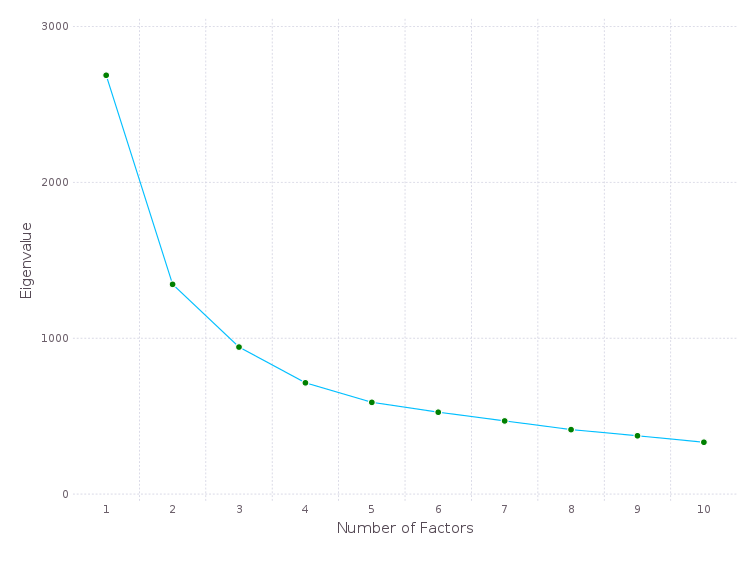
\includegraphics[width=10cm]{graphs/screeplot.png}
\caption{Scree plot of the eigenvalues calculated on the whole data set}
\label{screeplot}
\end{figure}


The first factor is most strongly correlated with variables related to total US output and manufacturing. Namely the $X_i$ with a large absolute correlation with the first factor are "Industrial Production Index", "Industrial Production: Durable Manufacturing (NAICS)", "Industrial Production: Manufacturing (NAICS)", "ISM Manufacting: PMI Composite Index", "ISM Manufacturing Production Index" and "Capacity Utilization: Total Industry".
The second factor mostly affects variables dealing with US construction and private housing: "Housing Starts in Midwest Census Region", "Housing Starts: Total: New Privately Owned Housing Units Started", "New Privately-Owned Housing Units Authorized by Building Permits: Total" and "All Employees: Construction". The second factor is also correlated with some output related variables in Germany such as "Output in the production sector", "Orders received" but also "Orders received" of the German construction industry.
For the third and the fourth factors the correlations are less strong in absolute variables but one can perhaps say that they are mostly correlated to hours worked and total employment variables in the US. 

All in all, these results reflect the relative importance of US business cycles for the chosen set of macroeconomic variables which can on the one hand be explained by the fact that $120$ of the $169$ variables are composed of US macroeconomic variables but on the other hand due to the relative sizes of the economies it is more likely that US variables affect German variables and thus that they have a higher influence on the underlying factors driving the evolution of the set of $X_i$. \\


If the number of static factors in the forecasting equation is predetermined using criteria defined above, the number of lags of the variable of interest $y_t$ and the number of lags of the static factors are still open. In the following I refer to the number of lags of $y_t$ as $s$. 

I follow \citet{bai2008forecasting} in selecting among model candidates using the BIC and the FPE criterion which are of course in-sample criteria. 

\citet{bai2008forecasting} write the BIC and FPE criteria as follows

\begin{equation}
\label{information criteria}
\begin{split}
	& \text{BIC} = \log(\hat \sigma_n^2) + n \frac{\log T}{T} \\ 
	& \text{FPE} = \log(\hat \sigma_n^2) + n \frac{2}{T}
\end{split}
\end{equation}

Where $\hat \sigma_n^2$ is the residual variance $\hat e'e$ from an estimation of the factor equation using $n$ predictors.

Since the point of the exercise is forecasting, additionally, the optimal model in terms of out-of-sample forecasting performance is found. This is done by calculating the root mean squared error of one step ahead pseudo out-of-sample forecasts.\footnote{Pseudo out-of-sample forecasts are a method to simulated a forecasting situation in that the forecaster does as if he would not know the true realizations of the data after $t$. The forecaster tries to predict the value $y_{t+h}$ given all the information up to $t$. $t$ is then successively moved one period ahead. Here we set $h=1$.} This evaluation method follows \citet{forni2005the} and \citet{bai2008forecasting} among others. The foreacasting window $w$ over which the pseudo out-of-sample-forecasts are performed is set to $w=15$ here. 

This forecasting window makes sure that there are more observations than parameters for all possible models. Since the length of the data series is $T=82$ this leaves $67$ observations for the first forecast in the pseudo out-of-sample procedure. The maximum number of factors is set to $15$ for static models and $10$ for dynamic models. The maximum number of lags of $y_t$ is set to $10$. This brings the maximal number of parameters to $n_{max} = 25$ for static models and $n_{max} = 50$ for dynamic models. The original number of predictors is $N = 169$ which highlights that factor models can be used as a dimensionality reduction method and that they are are an appropriate way to deal with the situation of $N>>T$ in this data set.
\\

All models are compared to a benchmark model which consists of a simple moving average of the $w$ periods before period $t+h$ which is being forecasted. The window size for the moving average benchmark is the same as the forecasting window $w$. 

The first panel in table \ref{results static factor model} shows the results of the in sample selection procedure for a static factor model. Three variants for choosing the number of factors are considered. Firstly the IC$_{p2}$ criterion from \citet{bai2002determining} is used to estimate the number of static factors for both the factor equation and the forecasting equation. The information criteria (BIC and FPE) are then used to select $s$, the number of lags of $y_t$.
As a second choice, the decision over the number of factors \textit{and} the number of lags of $y_t$ in the forecasting equation are left to the information criteria. I.e. the information criteria are minimized over different choices of $r$ and $s$. The same number of factors is used in the factor equation.
A third possibility consists of leaving the choice of the number of factors for the factor equation to a \citet{bai2002determining} criterion and using the BIC or FPE criterion to choose the number of static factors in the forecasting equation along with the number of lags of $y_t$. I.e. the BIC or FPE are minimized over $r$ and $s$.

Both the BIC and FPE as well as the $IC_{p2}$ criteria select a large number of factors and are generally very erratic in their choice of a model. The fact that conventional information criteria should not be used for selecting the number of static factors has been extensively documented in the factor model literature and is no surprise. Another approach to model selection for forecasting consists of testing the model in an out-of-sample forecasting situation and selecting the best performing model in terms of the forecasting error. In a forecasting application this would imply that a certain fraction of the data has to be used for 

The results of optimal forecasting model are reported in the second panel of table \ref{results static factor model}.

Since the variance of the data series has been normalized to $1$ and the mean to $0$ the RMSE of the simple average $y_t$ in the given window can be expected to be close to $1$. The RMSE of the resulting out-of-sample forecasts is very large with $1.30$ and $1.22$ respectively. The benchmark model of a moving average reports an RMSE of $0.86$ and an AR(6) model achieves an RMSE of $0.50$ for the same time horizon.\footnote{$p=6$ is the optimal lag number in terms of RMSE.}

The best performing static factor model in terms of forecasting can be got if the BIC criterion for model selecting is replaced by the RMSE as can be seen in the second panel. I.e. the RMSE is minimized over choices of $r$ and $s$ rather than the BIC. This implies using the out-of-sample performance as an evaluation criterion. In that case both $r$ and $s$ are shrunken to $1$. While this outperforms the simple benchmark model in form of the moving average, the fact that the most parsimonious static factor model performs best in out-of-sample prediction hints at possible performance increases if dynamic effects are allowed. It is interesting to consider why the AR(6) model outperforms the static factor model with an RMSE of about $0.50$ compared to $0.71$. The static factor model does not allow for a dynamic interaction between the factors and the dependent variable. In other words the factors can only influence the $X_i$ contemporaneously. As will be seen below, the dynamic factor model can improve on this result by allowing non-contemporaneous interaction.

\begin{table}[htp]
\centering
\caption{Static factor model, model selection}
\label{results static factor model}
\begin{tabular}{c|llll}
  & $r_{factor}$ & $r_{forecast}$ & $s$ & RMSE\\
  \hline
  \hline
    & \multicolumn{3}{l}{\textit{In-Sample}} \\
	BIC & 13 & 13 & 5 & 1.29 \\
	FPE & 15 & 15 & 5 & 1.23 \\
	$IC_{p2}$ \& BIC & 4 & 13 & 5 & 1.30 \\
	$IC_{p2}$ \& FPE & 4 & 15 & 5 & 1.23 \\
	$IC_{p2}$ & 4 & 4 & 10 & 1.21 \\
  \hline
  \hline
  & \multicolumn{3}{c}{\textit{Out-of-Sample}} \\ 
   	RMSE & 1 & 1 & 1 & 0.71 \\
   	RMSE \& $IC_{p2}$ & 4 & 1 & 1 & 0.72 \\
  \hline
  \multicolumn{5}{l} {\rule{0pt}{2.5cm} \begin{minipage}{8cm}
		\small{\textbf{\textit{Notes:}} The results are derrived by minimizing the criteria in the first column. If both an \citet{bai2002determining} criterion and a standard information criterion is given the former is applied to the factor equation and the latter to the forecasting equation. The maximum number of factors $r$ is set to $15$. The maximum number number of the lags of the variable of interest $s$ is set to $10$.}
  \end{minipage}} \\
\end{tabular}
\end{table}



Repeating the exercise but allowing for lags of the factors to enter the forecasting equation, the results in table \ref{results dynamic factor model} are obtained.\footnote{Essentially, table \ref{results static factor model} uses the same models as are used in table \ref{results dynamic factor model} with the added restriction $q=0$ and the fact the maximal number of factors has been reduced to $10$ because the factors enter the forecasting equation also in lagged form now which increases the number of parameters of the model quickly.} Since the data used for the exercise consists of time-series it makes sense that a dynamic factor model is better suited for prediction here. In the case of the dynamic model the FPE criterion readily selects too many parameters which results in a higher RMSE. The $IC_{p2}$ criterion chooses $r=4$ for the factor equation. For the forecasting equation, however, it seems to be better to increase the number of factors if the factors are also lagged in the forecasting equation. If the choice of the number of factors in both the factor and the forecasting equation is left to the IC$_{p2}$ which sets $r=4$, the RMSE increases to about $0.70$ as compared to $0.55$ if only $2$ factors, $3$ lags of the dependent variable and $1$ factor lag is chosen.

Also in this situation it does not necessarily make a difference in terms of RMSE if the number of factors differs in the factor equation and in the forecasting equation. This can be seen as in the optimal out-of-sample models they differ in both the static and the dynamic model while the RMSE stays the same. This no surprise as factor models relying on principal component estimation contain the most information in terms of variance in the first few factors.

In both the static and the dynamic factor model, choosing the number of static factors $r_{factor}$ in the factor equation using the IC$_{p2}$ criterion outperforms the other methods in terms of forecasting accuracy. Looking at table \ref{results dynamic factor model} it becomes clear why this is the case. Comparing panels a) and b) it is evident that the maximum number of factors, factor lags and lags of the dependent variable has to be chosen somewhat conservatively or else the model with the maximal number of factors and factor lags will be chosen. This is because the residuals are very small in these cases. If the number of factors is set by the IC$_{p2}$ criterion, the residuals are set "exogenously" to be big enough for the information criteria to perform well.

\begin{table}[ht]
	\centering
	\subfloat[Maximum number of factor lags $q$ set to 3]{
		\begin{tabular}{c|lllll}
		  & $r_{factor}$ & $r_{forecast}$ & $s$ & $q$ & RMSE\\
		 \hline
		 \hline
	     & \multicolumn{4}{l}{\textit{In-Sample}} \\
			BIC & 2 & 2 & 3 & 1 & 0.55 \\
			FPE & 10 & 10 & 10 & 3 & 2.91 \\
			$IC_{p2}$ \& BIC & 4 & 2 & 3 & 1 & 0.55 \\
			$IC_{p2}$ \& FPE & 4 & 10 & 10 & 3 & 2.91 \\
			$IC_{p2}$ & 4 & 4 & 10 & 2 & 0.70 \\
		  \hline
		  & \multicolumn{3}{c}{\textit{Out-of-Sample}} \\ 
		   	RMSE & 7 & 7 & 1 & 3 & 0.47 \\
		   	RMSE \& $IC_{p2}$ & 4 & 7 & 1 & 3 & 0.47 \\
		  \hline
		\end{tabular}
	} \\
%TODO: The following table is crap
	\subfloat[Maximum number of factor lags $q$ set to 4]{
		\begin{tabular}{c|lllll}
		  & $r_{factor}$ & $r_{forecast}$ & $s$ & $q$ & RMSE\\
		 \hline
		 \hline
 	     & \multicolumn{4}{l}{\textit{In-Sample}} \\
			BIC & 10 & 10 & 10 & 4 & 19.16 \\
			FPE & 10 & 10 & 10 & 3 & 19.16 \\
			$IC_{p2}$ \& BIC & 4 & 10 & 10 & 4 & 19.16 \\
			$IC_{p2}$ \& FPE & 4 & 10 & 10 & 4 & 19.16 \\
			$IC_{p2}$ & 4 & 4 & 10 & 4 & 0.78 \\
		  \hline
		  & \multicolumn{3}{c}{\textit{Out-of-Sample}} \\ 
		   	RMSE & 7 & 7 & 1 & 3 & 0.47 \\
		   	RMSE \& $IC_{p2}$ & 4 & 7 & 1 & 3 & 0.47 \\
		  \hline
		\end{tabular}	
	}

	\begin{minipage}{15cm}
		\small{\textbf{\rule{0cm}{6ex}
	\textit{Notes:}} The results are derrived by minimizing the criteria in the first column. If both a \citet{bai2002determining} criterion and a standard information criterion is given the former is applied to the factor equation and the latter to the forecasting equation. The maximum number of factors $r$ is set to $10$. The maximum number number of the lags of the variable of interest $s$ is set to $10$. $q$ here refers to the number of lags of the factors in the forecasting equation, not to the number of dynamic factors as defined above. The maximum number of the factor lags $q$ is set to 3 and 4 respectively. The results using the traditional information criteria hinge on the maximum number of factor lags.}
	\end{minipage}
	\caption{Dynamic factor model, model selection}
	\label{results dynamic factor model}
\end{table}
\clearpage


\subsection{Introducing structural breaks}
Structural breaks are estimated using Quandt-Andrews type supremum tests as defined above. The critival values for the test statistics are given in table I of \citet{andrews2003tests}. The number of estimated breaks per period can be seen in table \ref{breaks per period}.

It is apparent that there are two periods with major changes in the loadings. Firstly, there are structural breaks reported in the loadings of $8$ variables in the first quarter of 1999 which coincides approximately with the Russian default of 1998 and maybe the aftermath of the Asian financial crisis in 1997. In the following this period will be referred to as the first cluster of structural breaks. Secondly, a total of $22$ changes in the loadings are reported for the period of the second quater of 2008 until the second quarter of 2009 which coincides with the recent financial crisis starting after an US housing bubble burst. This period will be referred to as the second cluster of structural breaks. It caused and was affected by severe macroeconomic changes which are quite obviously reflected in the given data set. \\

Variables with breaks in the periods around 2008 include several aggregate variables which deal with orders received by German companies, variables describing productivity and total output, variables describing the monetary base and loans given by banks, the consumer price index, the market rates for treasury bills of differing maturities and the "University of Michigan Consumer Sentiment" survey. These are all variables which can be expected to undergo structural breaks during the 2008 financial crisis. Eminently, "PERMITNSA" which counts the number of new privately-owned housing units authorized, undergoes a structural break in the third quarter of 2005. This is also the time when the housing bubble in the US was arguably at its peak in terms of housing price increases: \citet{bernanke2010monetary} stresses that "[...] the most rapid price gains were in 2004 and 2005, when the annual rate of house price appreciation was between 15 and 17 percent". \\

Variables with breaks in the loadings at the first quarter of 1999 include German government debt, German exports and other trade related variables as well as variables describing bank term sheets and additionally, employment in the US durable goods sector.


\begin{table}[ht]
\caption{Number of structural breaks per period}
\label{breaks per period}
\centering
\begin{tabular}{|lllllllllllll|}
	\hline
	96:1 & 96:3 & 97:2 & 97:3 & 98:2 & 98:4 & 99:1 & 99:2 & 00:1 & 00:2 & 00:3 & 01:1 & 01:2 \\ 
	 2 & 1 & 2 & 1 & 1 & 1 & 8 & 1 & 1 & 2 & 1 & 3 & 1 \\
	\hline
	\hline
	03:2 & 04:3 & 04:3 & 05:1 & 05:2 & 05:3 & 07:1 & 07:2 & 07:3 & 07:4 & 08:1 & 08:2 & 08:3 \\
	1 & 1 & 2 & 1 & 1 & 1 & 1 & 1 & 1 & 1 & 1 & 4 & 2 \\
	\hline
	\hline
	 08:4 & 09:1 & 09:2 & 09:3 & 09:4 & 10:1 & & & & & & & \\
	 7 & 7 & 2 & 1 & 1 & 3 & & & & & & & \\
 	\hline

	\multicolumn{13}{l} {\rule{0pt}{6ex} \begin{minipage}{14.5cm}
		\small{\textbf{\textit{Notes:}} The entries show how many of the $N=169$ variables are predicted to undergo a structural break in each period. Reported are the numbers of significant values of $\mathscr{S}_{i,T}$ at the $5\%$ significance level. The total number of structural breaks found in the $169$ variables is $64$.}
	\end{minipage}} \\
\end{tabular}
\end{table}


\begin{figure}[htp]
\centering
\label{structural breaks per period}
\caption{Structural breaks per quarter}
\subfloat[5\% significance level]{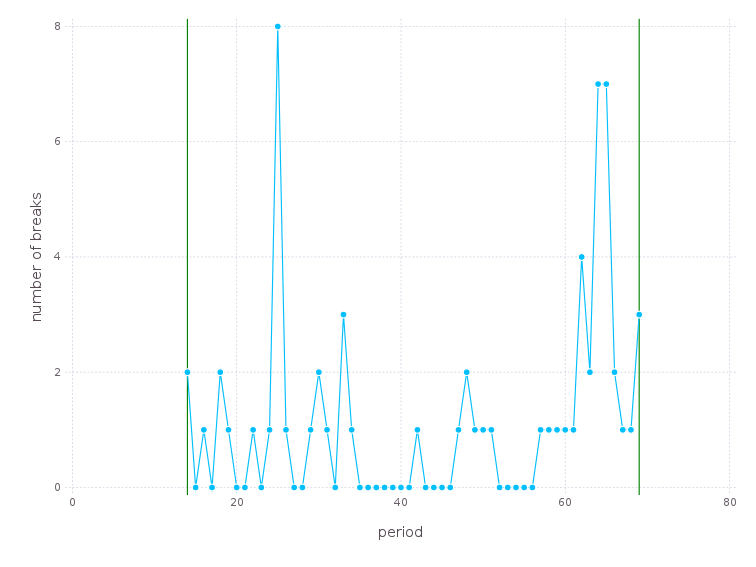
\includegraphics[width=8cm]{graphs/structural_breaks.png}}
\subfloat[1\% significance level]{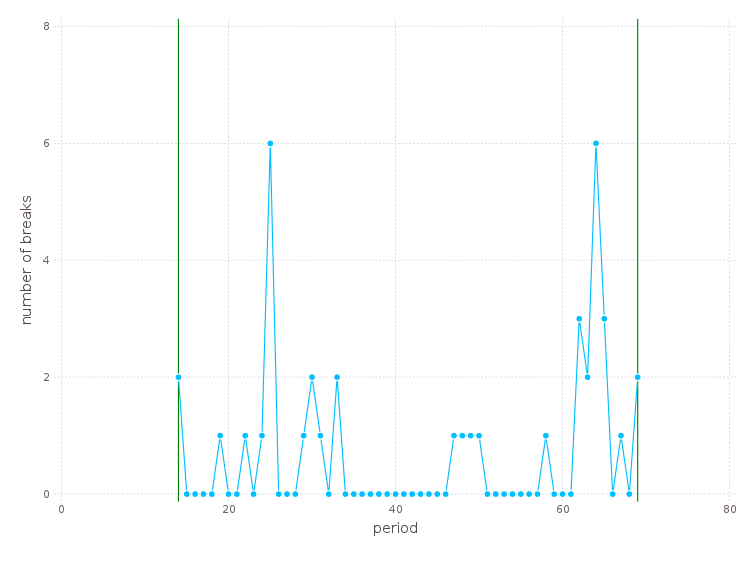
\includegraphics[width=8cm]{graphs/structural_breaks_1percent.png}}
\end{figure}

\subsubsection{Removing variables which undergo structural breaks}

In the following the question of how to react to the presence of structural breaks is approached as in section 2 above. Structural breaks in the factor loadings influence the performance of the forecasting equation through at least two channels. Firstly the presence of structural breaks decreases the signal to noise ratio in the data and thus the quality of the affected predictors. Secondly, \citet{breitung2011testing} show that it is necessary to increase the number of factors $r$ under the presence of structural breaks in order to estimate the space spanned by the factors. If the number of static factors in the forecasting equation is set equal to the number of static factors in the factor equation it becomes necessary to estimate a bigger number of parameters which can be an issue of practical relevance as has been seen above.


Either the length of the series is reduced by estimating the model only on data which is not subjected to structural breaks or the width of the data is reduced by removing the variables which are subjected to the structural break or a combination thereof. For the purpose of this paper we are interested in forecasting performance of factor models which ignore structural breaks versus factor models which take the structural breaks into account. Thus the results of models which restrict the amount of data to reduce the effect of structural breaks are compared with those that do not. It is worth noting that the comparison is not perfect because as has been argued in section $2$ it can be better to reduce the number of predictors to a set which is "targeted" towards the prediction of the variable of interest. It is possible that removing the variables with structural breaks "accidentally" targets the set of variables towards predicting the variable of interest independent of the structural break. In other words an improved result is not necessarily only due to the structural breaks being removed but might be due to a noisy predictor being removed. To be precise a series with a structural break could be considered a noisy predictor as well. However, it might be noisy independent of the structural breaks.
Resultingly, a robustness check consists of targeting the set of variables for both approaches prior to the estimation to remove that effect.

A practical difficulty has to be addressed before the results are presented. Given the fact that there are two periods where a majority of structural breaks occur, each of which affects a different set of factor loadings, cutting off the values before the significant break periods would leave very few observations for estimating the new model.

If both periods with major structural breaks are treated in a way that only data after the structural breaks is used, this would leave at most $17$ observations of which another $15$ have to be removed for the first step in the pseudo out-of-sample forecasts.

In principle there is a simple way to overcome this issue. It can be remembered that some of the data columns are monthly series which have been merged into the quarterly data set by dropping two thirds of the observations. The data could be cast back into monthly form. Most of the series will have missing data which can be interpolated (e.g. GDP is only reported quarterly). While this method solves the problem in a technical sense\footnote{For the first step of the pseudo out-of-sample period there are only $8$ data points for estimation. For every quarterly step of the pseudo out-of-sample procedure there are an additional $3$ observations. Thus, the ratio of observations to predictors improves quickly with each step of the pseudo out-of-sample prediction.}, it has several drawbacks: firstly no additional information is added by the interpolation although there are more observations available to the model. At the same time the imputation adds additional uncertainty. Traditional standard error estimates do not account for this and resultingly they may be downward biased (cf. \citet[chapter~25]{gelman2006missing}. It is thus likely that prediction based on this short data set performs badly in a forecasting sense. On the other hand, if predictions resulting from this shaved data set should perform better, it would constitute a strong indication that the structural breaks uncovered by the tests should not be ignored. In this case doing so clearly leads to a significant degradation of forecasting results. This has not been tested here. 

Instead four approaches to removing the effects of structural breaks from the data are considered. First the variables in the second cluster of structural breaks between the second quarter of 2008 and the first quarter of 2009 are removed. Because this approaches ignores the first cluster of structural breaks in the first quarter of 1999, a second model is estimated to explore what happens if these series are excluded as well. A third model removes all series with structural breaks in the loadings. Finally, the fourth model leaves the \textit{variables} with breaks in the first cluster in 1999 in the model but removes \textit{observations} prior to the second quarter of 1999. 

For all four approaches the best performing dynamic factor model in terms of RMSE is reported where the number of static factors in the factor equation is calculated using the IC$_{p2}$ criterion and the number of factors in the forecasting equation as well as the number of factor lags is chosen according to the minimum of the RMSE of out-of-sample forecasts. Structural breaks are detected at the $5\%$ significance level.

The figures in appendix \ref{structural breaks, reduced data sets} show the number of significant structural breaks left if the above adjustements to the data have been made. The reason to check for structural breaks again after some variables have been removed or the observations prior to the second quarter of 1999 have been removed, is that the estimation of the factor equation changes with a reduced set of variables which has an impact on the statistics of the structural break tests.

Table \ref{results dynamic factor model, reduced data sets} shows that the exclusion of variables improves the RMSE considerably compared to ignoring the structural breaks. For this data set, the more variables with structural breaks at the 5\% significance level are removed, the lower the RMSE becomes.

\begin{table}[ht]
	\centering
	\begin{tabular}{c|lllll}
		   & $r_{factor}$ & $r_{forecast}$ & $s$ & $q$ & RMSE \\
		 \hline
		 \hline
		    & & \multicolumn{3}{c}{\textit{Second break cluster removed}} \\
			& & \multicolumn{3}{c}{$T=82, N=149$} \\
		  \hline
		   	RMSE & 7 & 7 & 1 & 3 & 0.45 \\
		   	RMSE \& $IC_{p2}$ & 3 & 7 & 1 & 3 & 0.45 \\
		  \hline
		  \hline
		  & \multicolumn{5}{c}{\textit{First and second break cluster removed}} \\ 
			& & \multicolumn{3}{c}{$T=82, N=141$} \\
		  \hline
		   	RMSE & 6 & 6 & 4 & 2 & 0.44 \\
		   	RMSE \& $IC_{p2}$ & 3 & 6 & 4 & 2 & 0.44 \\
		  \hline
		  \hline
	  	  & \multicolumn{5}{c}{\textit{All variables with breaks removed}} \\ 
			& & \multicolumn{3}{c}{$T=82, N=105$} \\
          \hline
		   	RMSE & 6 & 6 & 3 & 2 & 0.40 \\
		   	RMSE \& $IC_{p2}$ & 3 & 3 & 4 & 2 & 0.39 \\
		  \hline
		  \hline
		  & \multicolumn{5}{c}{\textit{Second break cluster removed, length trimmed}} \\
			& & \multicolumn{3}{c}{$T=57, N=149$} \\
		  \hline
		   	RMSE & 1 & 1 & 5 & 1 & 0.51 \\
		   	RMSE \& $IC_{p2}$ & 4 & 1 & 5 & 1 & 0.51 \\
		  \hline
		  \hline		  
	\end{tabular}
	\caption{Dynamic factor model, data adjusted for structural breaks}
	\label{results dynamic factor model, reduced data sets}
\end{table}


Figures for the number of structural breaks per period after variables have been dropped or the data length has been trimmed can be found in appendix \ref{structural breaks, reduced data sets}. Notably figure \ref{reduced data set, all variables with breaks removed} shows a modest number of structural breaks at the 5\% significance level \textit{after} all structural breaks had been removed from the data set. Iterating the procedure by removing the variables with structural breaks again increases the RMSE to $0.72$ which makes clear that blindly removing all variables which contain structural breaks need not be a good idea even though the previous results in table \ref{results dynamic factor model, reduced data sets} seemed to indicate that removing as many variables with structural breaks as possible has a positive effect on RMSE.


\subsubsection{Removing variables with breaks after targeting the data}
It was found before that removing all variables with structural breaks can improve the forecasting performance. To test if targetting the predictors and removing the structural breaks has a similar effect, the variables with structural breaks are removed after the data set has been targeted. To this end the following sub section considers the residual effect of removing the structural breaks after the effect of targeting the predictors has been accounted for. Both soft and hard thresholding rules are applied.

It should be noted as well that German GDP, -the variable of interest is included in the set of dependent variables in the factor equation (\ref{factor equation}) (as is customary) and breaks are sometimes detected in the factor loading of this variable if the data set is targeted. German GDP is still kept in the data set in all variable pre-selection schemes even if all other variables with breaks are removed from the set.

Starting with hard thresholding, targeting the predictors at the 10\%, 5\% and 1\% significance level (see \citet{bai2008forecasting} for details) leaves $85$, $78$ and $43$ variables in the data set respectively. Figure \ref{structural breaks per period, targeted predictors} shows that targetting the data removes a part of the two clusters of structural breaks found in the original data. It can be inspected in table \ref{results dynamic factor model, targeted data sets} that with hard thresholding the RMSE is higher than it was for the best performing model of the original data set. For the complete data set the optimal model achieved an RMSE of $0.47$. with hard thresholding the RMSE increases to about $0.50$ for all three cut-off values. Regardless of the relatively bad performance of hard thresholding rules to target the predictors, removing the structural breaks from the targeted data set marginally improves the results.

\begin{table}[ht]
	\centering
	\begin{tabular}{c|lllll}
		   & \multicolumn{4}{c}{\textbf{Hard thresholding}} \\
		   & $r_{factor}$ & $r_{forecast}$ & $s$ & $q$ & RMSE\\
		 \hline
		 \hline
		  & \multicolumn{5}{c}{$\alpha=0.1$} \\ 
		  & \multicolumn{5}{c}{$T=82, N=85$} \\
		  \hline
		   	RMSE & 1 & 1 & 5 & 2 & 0.50 \\
		   	RMSE \& $IC_{p2}$ & 6 & 1 & 5 & 2 & 0.50 \\
		 \hline
 		 \hline
		  & \multicolumn{5}{c}{Hard Thresholding $\alpha=0.05$} \\ 
 		 & \multicolumn{5}{c}{$T=82, N=78$} \\
		  \hline
		   	RMSE & 1 & 1 & 5 & 2 & 0.50 \\
		   	RMSE \& $IC_{p2}$ & 6 & 1 & 5 & 2 & 0.50 \\
		 \hline
 		 \hline
 		 & \multicolumn{5}{c}{$\alpha=0.01$} \\ 
 		 & \multicolumn{5}{c}{$T=82, N=43$} \\
		  \hline
		   	RMSE & 1 & 1 & 5 & 2 & 0.49 \\
		   	RMSE \& $IC_{p2}$ & 7 & 1 & 5 & 2 & 0.49 \\
		 \hline
 		 \hline
	\end{tabular}
	\caption{Dynamic factor model, targeted data, hard thresholding}
	\label{results dynamic factor model, targeted data sets}
\end{table}

\begin{table}[ht]
	\centering
	\begin{tabular}{c|llllll}
		   & \multicolumn{5}{c}{\textbf{Hard thresholding, breaks removed}} \\
		   & $r_{factor}$ & $r_{forecast}$ & $s$ & $q$ & RMSE & $\Delta$ \\
		 \hline
		 \hline
		    & \multicolumn{5}{c}{$\alpha = 0.1$} \\ 
			& \multicolumn{5}{c}{$T=82, N=51$} \\
		  \hline
		   	RMSE & 11 & 11 & 2 & 1 & 0.44 & 0.06 \\
		   	RMSE \& $IC_{p2}$ & 4 & 11 & 2 & 1 & 0.44 & 0.06\\
		 \hline
		 \hline
		    & \multicolumn{5}{c}{$\alpha = 0.05$} \\ 
			& \multicolumn{5}{c}{$T=82, N=51$} \\
		  \hline
		   	RMSE & 1 & 1 & 5 & 2 & 0.50 & 0 \\
		   	RMSE \& $IC_{p2}$ & 4 & 1 & 5 & 2 & 0.50 & 0\\
		 \hline
 		 \hline
 		    & \multicolumn{5}{c}{$\alpha = 0.01$} \\ 
			& \multicolumn{5}{c}{$T=82, N=28$} \\
		 \hline
			& \multicolumn{5}{c}{Results omitted} \\

		 \hline
 		 \hline
 		 
		 \multicolumn{7}{l} {\rule{0pt}{3.5cm} \begin{minipage}{12cm}
			\small{\textbf{\textit{Notes:}}  $T$ and $N$ denote the dimension of the targeted data sets where all variables with evidence of structural breaks found at the 5\% level using the sup LM test have been removed. The column denoted with $\Delta$ calculates the difference between the RMSE of the best factor model calculated on the targeted data with structural breaks removed and the results from table \ref{results dynamic factor model, targeted data sets} where the structural breaks have not been removed. Note that the set of variables for hard thresholding with $\alpha=0.05$ differs although the number of variables coincides. Also note that there are no results for $\alpha=0.01$ because the estimated number of factors for this data set is $22$ for wich there are no tabulated values to calculate the structural break tests with in \citet{andrews2003tests}. The critical values have not been simulated here.}
		 \end{minipage}} \\
	\end{tabular}
	\caption{Dynamic factor model, targeted data, structural breaks removed}
	\label{results dynamic factor model, reduced targeted data sets}
\end{table}


\begin{figure}[htp]
\centering
\subfloat[5\% significance level]{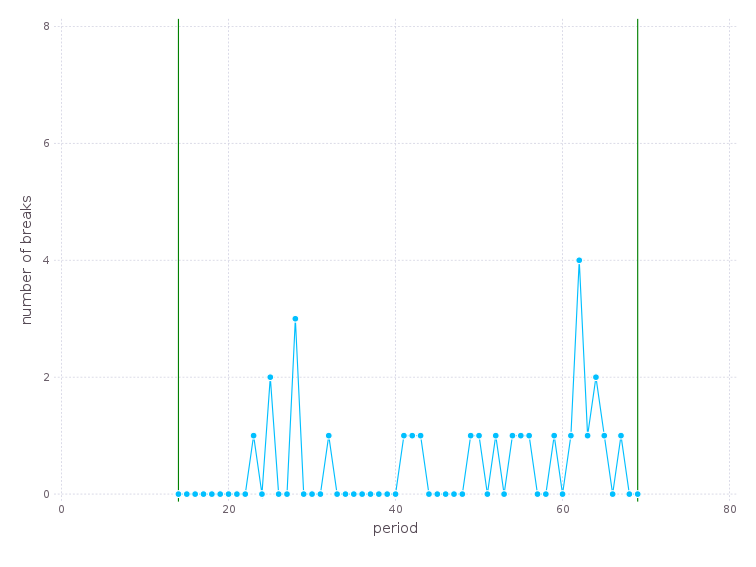
\includegraphics[width=8cm]{graphs/structural_breaks_targeted.png}}
\subfloat[1\% significance level]{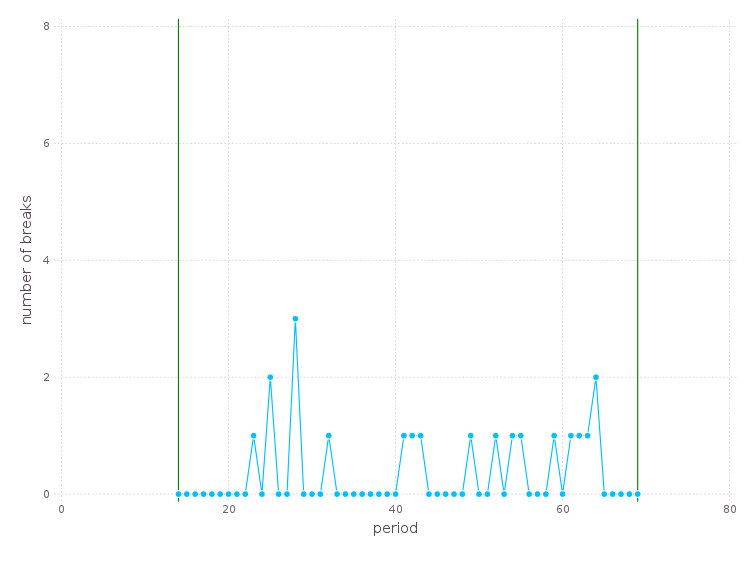
\includegraphics[width=8cm]{graphs/structural_breaks_targeted_1percent.png}}
\caption{Structural breaks per quarter, targeted predictors}
\label{structural breaks per period, targeted predictors}
\end{figure}



\clearpage

As noted in the introduction on targeted predictors above, the difficulty with soft thresholding lies in the choice of the number of steps $k$ in the LARS-EN algorithm. This coincides with the number of variables chosen as each step adds one variable to the active set. It is conceivable that if the thresholding is too strict, i.e. the regularization parameter too large, the LASSO will have kicked out most of the variables which contain structural breaks. A chosen set of results of the removal of structural breaks after applying soft thresholding using the LASSO can be seen in table \ref{results dynamic factor model, targeted data sets, soft thresholding}. 

The value of $k$ which yields the best performing targeted predictor model is $k=39$ which gives an RMSE of just below $0.4$ as can be inspected in table \ref{results dynamic factor model, targeted data sets, soft thresholding}. The fact that the maximum number of factors is chosen is suspicious. However, if the maximum number of factors is increase the results remain constant. The same holds for $k=30$ and for the number of factor lags. \\


\begin{table}[ht]
	\centering
	\begin{tabular}{c|llllll}
		   & \multicolumn{5}{c}{\textbf{Soft thresholding}} \\
		   & $r_{factor}$ & $r_{forecast}$ & $s$ & $q$ & RMSE & $\Delta_\text{RMSE}$ \\
		 \hline
		 \hline
		  & \multicolumn{6}{c}{$k=39$} \\ 
		  & \multicolumn{6}{c}{$T=82, N=39$} \\
		  \hline
		   	RMSE & 15 & 15 & 3 & 1 & 0.4000 & $-0.0811$ \\
		   	RMSE \& $IC_{p2}$ & 2 & 15 & 3 & 1 & 0.4000 & $-0.0811$\\
		 \hline
 		 \hline
		  & \multicolumn{6}{c}{$k=32$} \\ 
 		  & \multicolumn{6}{c}{$T=82, N=32$} \\
		  \hline
		   	RMSE & 13 & 13 & 1 & 1 & 0.4014 & $-0.0125$ \\
		   	RMSE \& $IC_{p2}$ & 2 & 13 & 1 & 1 & 0.4014 & $-0.0125$\\
		 \hline
 		 \hline
 		  & \multicolumn{6}{c}{$k=40$} \\ 
 		  & \multicolumn{6}{c}{$T=82, N=40$} \\
		  \hline
		   	RMSE & 15 & 15 & 3 & 1 & 0.4141 & $-0.0716$ \\
		   	RMSE \& $IC_{p2}$ & 2 & 15 & 3 & 1 & 0.4141 & $-0.0716$ \\
		 \hline
 		 \hline
		\multicolumn{7}{l} {\rule{0pt}{1cm} \begin{minipage}{11cm}
			\small{\textbf{\textit{Notes:}} The entries report detailed results of the three best performing optimal models for $k \in \{30, 32, 39\}$. Less detailed results for more values of $k$ can be found in table \ref{diff rmse by removing breaks after targeting} in the appendix. $\Delta_\text{RMSE}$ denotes the change in RMSE if the optimal model is calculated from the targeted data set with variables containing structural breaks removed. The maximum number of factors is set to $15$, the maximum number of factor lags is set to $3$ and the maximum number of lags of $y_t$ is set to $5$}
		\end{minipage}} \\
	\end{tabular}
	\caption{Dynamic factor model, targeted data, soft thresholding}
	\label{results dynamic factor model, targeted data sets, soft thresholding}
\end{table}


The $39$ variables contained in the best performing targeted predictor model include German output and employment variables, several variables describing German exports and the trade balance. The US variables included contain output and employment variables, some production related financial variables such as "Commercial and Indstrial Loans", the consumer and producer price indices, construction and housing variables as well as monetary variables and the "6-Month Treasurey Bill: Secondary Market Rate". Interestingly the foreign exchange rate between Switzerland and the US is also added to the set of variables. It is likely that this variable captures the lack of other exchange rates in the data set.

The second best performing model removes some of the variables but because the second best model is nothing but an earlier point on the solution path, the other variables remain the same. The removed variables inlcude one of the German export variables, the US labor force participation rate, one of the US housing starts variables and markedly the producer price index.


Relative improvements of removing structural breaks for more values of $k$ and Diebold-Mariano test statistics\footnote{The models are estimated on different subsets of the data set. Strictly speaking the models could be seen as nested and another comparison procedure such as \citet{clark2001tests} should be used depending on the specificity of the restriction. This corner case is ignored here.} are shown in table \ref{diff rmse by removing breaks after targeting}. The table starts with $k=26$ which is the first value in the LASSO solution path for which the resulting number of factors calculated by the IC$_{p2}$ criterion returns sensible values.\footnote{Sensible here means smaller than $20$ which is the last value for which \citet{andrews2003tests} has tabulated critical values.}
It can be seen that removing the variables with structural breaks can only improve the RMSE for some of the different sets of targeted data. This can be seen in the positive entries in the $\Delta_{\text{RMSE}}$ column.

However, significant improvements in forecasting accuracy can only be confirmed for $k=49$ at customary levels of significance and different forecasting performance can only be detected for $3$ choices of $k$. It should also be noted that even this one rejection has to be taken with a grain of salt although significant at the 1\% level. This is because if the 5\% significance level is taken, at least one rejection can be expected due to chance in $25$ tests and at the 1\% level $1$ false rejection is less likely but possible nonetheless.



\clearpage

To further study the interaction between targeted predictors and structural breaks in a confined environment, in a final step, a monte carlo study is performed in which the simulated data contains a structural break in only one of the factor loadings. The size of the break and the information content for the prediction of $y$ is varied in one predictor. The idea is to meassure the difference in RMSE in this contained environment if the variable is removed versus keeping the variable in the model for varying sizes of the break and levels of information for predicting $y$. More precisely the Cholesky decomposition is used in order to generate data with varying degree of dependence $\delta$ between the dependent variable and the predictor which experiences a structural break of size $b$. All values of $\delta$ which are bigger than $0.1$ imply that the last column is typically chosen first if the predictors are targeted.
Table \ref{montecarlo of DM-tests for varying break size and information} shows that a higher $\delta$ decreases the likelihood of an improved forecasting accuracy which is intuitive because removing an informative predictor should decrease performance. It seems that an increase in the break size $b$ has the same effect but this effect seems to be less pronounced.

\begin{table}[ht]
	\center{
		DGP: $X_{it} = \sum_{j=1}^r \lambda_{ij}F_{tj} + \text{chol}(v(\delta)) e_{it}, r=1$ \\
		\vspace{0.5cm}
		where $v(\delta)=   \begin{bmatrix}
			1 & 0.1 & \dots & \dots & 0.1 & \delta  \\
			0.1 & 1 & 0.1 & \dots & 0.1 & 0.1 \\
			\vdots & 0.1 & \ddots & 0.1 & \vdots & \vdots \\
			\vdots & \vdots & 0.1 & \ddots & 0.1 &  \vdots \\
			0.1 & \vdots & \vdots & 0.1 & \ddots & 0.1 \\
			\delta & 0.1 & \dots & \dots & 0.1 & 1 \\
	  \end{bmatrix}$
	} \\
	\vspace{0.5cm}
	\centering
	\begin{tabular}{cc|llllllllll}
		& & $\delta$ \\
		& & 0.1 & 0.2 & 0.3 & 0.4 & 0.5 & 0.6 & 0.7 & 0.8 & 0.9 & 0.99 \\
		\hline
			b & 0.0 & 0.040 & 0.036 & 0.018 & 0.020 & 0.024 & 0.024 & 0.020 & 0.018 & 0.014 & 0.028 \\
 			& 0.1 & 0.032 & 0.024 & 0.026 & 0.026 & 0.026 & 0.008 & 0.026 & 0.010 & 0.020 & 0.004 \\
 			& 0.2 & 0.026 & 0.020 & 0.020 & 0.024 & 0.018 & 0.018 & 0.018 & 0.014 & 0.014 & 0.008 \\
			& 0.3 & 0.042 & 0.040 & 0.020 & 0.008 & 0.014 & 0.020 & 0.010 & 0.024 & 0.022 & 0.002 \\
			& 0.4 & 0.040 & 0.036 & 0.020 & 0.026 & 0.020 & 0.008 & 0.010 & 0.026 & 0.010 & 0.018 \\
			& 0.5 & 0.030 & 0.028 & 0.022 & 0.016 & 0.016 & 0.018 & 0.020 & 0.018 & 0.014 & 0.008 \\
			& 0.6 & 0.040 & 0.040 & 0.014 & 0.012 & 0.004 & 0.016 & 0.030 & 0.004 & 0.008 & 0.012 \\
			& 0.7 & 0.042 & 0.036 & 0.020 & 0.028 & 0.014 & 0.020 & 0.018 & 0.016 & 0.010 & 0.012 \\
			& 0.8 & 0.036 & 0.034 & 0.024 & 0.016 & 0.024 & 0.016 & 0.018 & 0.016 & 0.006 & 0.010 \\
			& 0.9 & 0.030 & 0.034 & 0.018 & 0.014 & 0.026 & 0.014 & 0.014 & 0.014 & 0.010 & 0.012 \\
			& 1.0 & 0.028 & 0.024 & 0.016 & 0.012 & 0.020 & 0.026 & 0.012 & 0.020 & 0.020 & 0.018 \\
		\hline
		\multicolumn{12}{l} {\rule{0pt}{2.5cm} \begin{minipage}{15cm}
			\small{\textbf{\textit{Notes:}} The entries report the average rejection rate of $R=500$ Diebold-Mariano tests of improved forecasting performance at the 5\% significance level. The two competing models are static factor models, one of which includes the column with the structural break, the other does not. Optimal models are chosen using the RMSE as before. The structural break occurs in the mid observation $T^*=25$ in the last column. The size of the break is given by $b$ and the correlation of the dependent variable in the first column with last column is given by $\delta$. $T=50, N=20$}
		\end{minipage}} \\
	\end{tabular}
	\caption{Montecarlo of DM-tests for varying break size and information}
	\label{montecarlo of DM-tests for varying break size and information}
\end{table}


\clearpage
\section{Conclusion}
While factor models perform quite well in forecasting economic time-series, structural breaks can, if not accounted for, undermine the forecasting performance significantly. Not only does one have to be careful with the actual prediction results but also interpretting the factors directly can become unfeasible as the number of static factors changes under structural breaks.

Estimating different model specifications under structural breaks on a large macroeconomic data set including German and US macroeconomic variables shows that removing variables with structural breaks tends to improve forecasting accuracy considerably. In this data set the improvement of removing the variables which undergo structural breaks improves the performance more so than removing the pre-break observations. This result must not necessarily hold for different data sets and could be an artifact of its relative shortness.

The best performing models with breaks removed handily beat the best performing benchmark AR(p) model and the benchmark moving average model as well as dynamic factor models which do not account for breaks.

The best overall results are achieved using targeted perdictors with soft thresholding with $k=39$ which amounts to keeping only roughly 23\% of the original predictors.

The removal of variables which feature structural breaks works similarly to the method of targeted predictors. While each method individually improves forecasting precision, there is little evidence that the two methods used in conjunction further improve the forecasting results. This hints at a trade-off. The method of removing structural breaks ignores the information contained in the predictor while soft-thresholding focusses on correlatedness over the whole time-frame without taking into account that the linear relationship might break down over time. Put differently: as long as two predictors are sufficiently correlated \textit{overall} it does not matter if the most recent data follow a different data generating process if targeted predictors are used for variable pre-selection. Further research into variable pre-selection methods for factors models could also yield a method which generalizes targeted predictors and the approach to remove variables featuring structural breaks.

It should be noted that the approach to remove all variables which have significant structural breaks is very crude and comparatively unfair with respect to targeted data under soft thresholding because the latter consists of a whole solution path of which the best solution is picked. Alternatively and perhaps more fairly one could consider removing variables step by step starting e.g. with variables which have a high associated sup LM statistic. This is likely to yield additional gains in forecasting performance.

Additionally and independently from the treatment of structural breaks, the model selection framework can be further refined. It is likely for example that allowing factors to enter the forecasting equation with different lag levels can help to boost the forecasting performance.


\clearpage
\newpage
\appendix
\section*{Apendix}
\addcontentsline{toc}{section}{Appendix}

\section{Derrivation of Principal Components}
\label{Derrivation of Principal Components}
The principal components of a data matrix $X$ are defined as the transformation of $X$ into the space spanned by the loadings \footnote{The $u_i$ are also called scores or principal component directions.} $u_i$ where each $u_i$ is a unit vector. The transformation is defined such that the transformed columns are uncorrelated (as are the loadings $u_i$) and such that the first transformed column (i.e. the first principal component) contains the largest amount of the variance of the original data, the second column the second largest amount (i.e. the second principal component), etc. \\

Let $X$ have mean 0 (i.e. subtract the mean from each observation if it does not).
For the first principal component, we want to find a loading vector vector $u_1$ such that the variance along the projection of $x$ onto the first principal component direction $u_1$ is maximized where $u_1$ is a unit norm vector. 
$$\underset{u_1: ||u_1|| = 1}{\max} \ \frac{1}{T} \sum_{i=1}^T(x_i'u_1)^2 = \underset{u_1: u_1'u_1 = 1}{\max} \ u_1' ( \frac{1}{T} \sum_{i=1}^T x_i'x_i )u_1 = \underset{u_1: u_1'u_1 = 1}{\max} \ u_1' (\Sigma)u_1$$
Setting up the Lagrangian yields
$$ L(u_1, \lambda) = u_1' \Sigma u_1 - \lambda(u_1'u_1-1)$$
After taking the derivative with respect to $u_1$ and dividing by 2 we are left with
$$\frac{\partial L}{\partial u_1} = \Sigma u_1 -\lambda u_1 \overset{!}{=} 0$$ in other words $u_1$ is an eigenvector of $\Sigma$, the covariance matrix of x. The corresponding eigenvalue is $\lambda$ and we must have $\Sigma = \lambda$ for the variance of the principal component to be maximal under the constraint. \\
The maximal variance of $x'u_1$ is thus $V(x'u_1) = u_1' \Sigma u_1 = u_1' \lambda u_1$ and it is achieved for the highest eigenvalue $\lambda$ of the covariance matrix of x. The derrivation of the following principal components is accordingly subject to the additional constraint that the principal components are uncorrelated. In the case of the second principal component this implies $\text{cov}(u_1'x, u_2'x) = u_1' \Sigma u_2 = 0$. The solution for the third and all following principal component is more complex but goes accordingly. The derrivations can be seen e.g. in \citet{jolliffe2005principal} or any other textbook on the subject. The solution for the $i$-th principal component is to set the loadings $u_i$ to be eigenvector which belongs to the $i$-th highest eigenvalue. Also, for each principal component $i$ we get that $\text{var}(u_i'x) = \lambda_i$.

\newpage
\section{Estimation of the Factor Equation}
\label{Estimation of the Factor Equation}
Estimators of the factor equation solve (\ref{factor equation minimization problem}).
$$\min_{F_1, ..., F_T, \Lambda} V_r(\Lambda, F) = \min_{F_1, ..., F_T, \Lambda} \frac{1}{NT} \sum_{t=1}^T (X_t - \Lambda F_t)'(X_t - \Lambda F_t)$$

$$\text{s.t. } N^{-1} \Lambda' \Lambda = I_r$$

The solution can be gotten by first optimizing over $F_t$. The first order condition is: $$\frac{\partial V_r}{\partial F_t} = -2X'_t \Lambda + 2 \hat F'_t \Lambda' \Lambda \overset{!}{=} 0$$

Resultingly $\hat F_t = (\Lambda' \Lambda)^{-1} \Lambda' X_t$. Inserting that back into the optimization problem gives $\min_\Lambda \frac{1}{NT} X_t'X_t - 2X_t' \Lambda (\Lambda' \Lambda)^{-1} \Lambda'X_t + X_t' \Lambda (\Lambda' \Lambda)^{-1} \Lambda' \Lambda (\Lambda' \Lambda)^{-1} \Lambda'X_t = \min_\Lambda \frac{1}{NT} X_t' [I - \Lambda (\Lambda' \Lambda)^{-1} \Lambda']X_t$. \\
This is equivalent to the problem $\max_\Lambda \text{tr}\left\{(\Lambda'\Lambda)'^{-\frac{1}{2}}\lambda'(T^{-1} \Sigma_{t=1}^T X_tX_t') \Lambda (\Lambda' \Lambda)^{-\frac{1}{2}}\right\}$ which is the same as $\max_\Lambda \Lambda' \hat \Sigma_{XX} \Lambda \text{ s.t. } N^{-1} \Lambda' \Lambda = I_r$ where $\hat \Sigma_{XX}$ is the usual sample equivalent of the variance of $X$. This can be solved by setting $\hat \Lambda$ to eigenvectors of the $r$ largest eigenvalues of $\hat \Sigma_{XX}$.


\newpage
\section{Replication of \citet{bai2002determining} for $r=7$, $r=9$}

\label{bai ng information criteria}
\begin{table}[h!]
\caption{Replication of Table I of \citet{bai2002determining} for $r=7$}
\center{
	DGP: $X_{it} = \sum_{j=1}^r \lambda_{ij}F_{tj} + \sqrt{\theta}e_{it}, r=7$
} \\
\center
\begin{tabular}{cc|lllllll}

	N & T & $PC_{p1}$ & $PC_{p2}$ & $PC_{p3}$ & $IC_{p1}$ & $IC_{p2}$ & $IC_{p3}$\\
	\hline
		100 & 40 & 6.4 & 5.9 & 6.97 & 4.93 & 3.46 & 6.73 & \\ 
		100 & 60 & 6.72 & 6.27 & 7.02 & 6.34 & 4.74 & 6.99 & \\ 
		200 & 60 & 6.93 & 6.87 & 7.0 & 6.78 & 6.46 & 6.96 & \\ 
		500 & 60 & 6.99 & 6.96 & 7.0 & 6.94 & 6.92 & 6.99 & \\ 
		1000 & 60 & 7.0 & 6.99 & 7.0 & 6.99 & 6.97 & 7.0 & \\ 
		2000 & 60 & 7.0 & 6.99 & 7.0 & 6.98 & 6.99 & 7.0 & \\ 
		100 & 100 & 7.0 & 6.77 & 7.35 & 6.89 & 6.32 & 50.0 & \\ 
		200 & 100 & 7.0 & 7.0 & 7.0 & 7.0 & 6.99 & 7.0 & \\ 
		500 & 100 & 7.0 & 7.0 & 7.0 & 7.0 & 7.0 & 7.0 & \\ 
		1000 & 100 & 7.0 & 7.0 & 7.0 & 7.0 & 7.0 & 7.0 & \\ 
		2000 & 100 & 7.0 & 7.0 & 7.0 & 7.0 & 7.0 & 7.0 & \\ 
		40 & 100 & 6.39 & 6.12 & 7.02 & 4.86 & 3.49 & 6.78 & \\ 
		60 & 100 & 6.79 & 6.37 & 7.01 & 6.01 & 5.0 & 7.0 & \\ 
		60 & 200 & 6.93 & 6.85 & 7.0 & 6.82 & 6.58 & 6.98 & \\ 
		60 & 500 & 6.96 & 6.97 & 7.0 & 6.97 & 6.9 & 6.99 & \\ 
		60 & 1000 & 7.0 & 6.99 & 7.0 & 6.99 & 6.96 & 7.0 & \\ 
		60 & 2000 & 7.0 & 7.0 & 7.0 & 6.97 & 6.98 & 6.99 & \\ 
		4000 & 60 & 7.0 & 7.0 & 6.99 & 6.98 & 6.99 & 6.99 & \\ 
		4000 & 100 & 7.0 & 7.0 & 7.0 & 7.0 & 7.0 & 7.0 & \\ 
		8000 & 60 & 6.99 & 7.0 & 7.0 & 7.0 & 6.98 & 7.0 & \\ 
		8000 & 100 & 7.0 & 7.0 & 7.0 & 7.0 & 7.0 & 7.0 & \\ 
		60 & 4000 & 7.0 & 7.0 & 7.0 & 7.0 & 7.0 & 6.99 & \\ 
		100 & 4000 & 7.0 & 7.0 & 7.0 & 7.0 & 7.0 & 7.0 & \\ 
		60 & 8000 & 6.99 & 7.0 & 7.0 & 6.99 & 7.0 & 6.99 & \\ 
		100 & 8000 & 7.0 & 7.0 & 7.0 & 7.0 & 7.0 & 7.0 & \\ 
	\hline
		10 & 50 & 5.0 & 5.0 & 5.0 & 4.76 & 3.95 & 5.0 & \\ 
		10 & 100 & 5.0 & 5.0 & 5.0 & 4.58 & 4.18 & 4.96 & \\ 
		20 & 100 & 7.04 & 6.5 & 7.98 & 3.14 & 2.07 & 6.94 & \\ 
		100 & 10 & 5.0 & 5.0 & 5.0 & 5.0 & 4.96 & 5.0 & \\ 
		100 & 20 & 7.1 & 6.64 & 8.05 & 3.3 & 2.08 & 8.2 & \\ 
	\hline
	\hline
	\\
	\multicolumn{8}{l} {\begin{minipage}{9.5cm}
		\small{\textbf{\textit{Notes:}} Estimated number of factors averaged over 1000 simulations. The true number of factors is $r$ and the maximum number of factors is $\text{ceil}(\min\{T, N\})/2)$.}
	\end{minipage}} \\

\end{tabular}
\end{table}


\begin{table}[htp]
\caption{Replication of Table I of \citet{bai2002determining} for $r=9$}
\center{
	DGP: $X_{it} = \sum_{j=1}^r \lambda_{ij}F_{tj} + \sqrt{\theta}e_{it}, r=9$
} \\
\center{
	see \citet{bai2002determining} for specification of the DGP
}

\center
\begin{tabular}{cc|lllllll}
	N & T & $PC_{p1}$ & $PC_{p2}$ & $PC_{p3}$ & $IC_{p1}$ & $IC_{p2}$ & $IC_{p3}$\\
	\hline
		100 & 40 & 6.51 & 5.93 & 8.06 & 3.55 & 1.49 & 7.89 & \\ 
		100 & 60 & 7.02 & 6.25 & 8.77 & 5.4 & 2.74 & 8.9 & \\ 
		200 & 60 & 7.74 & 7.31 & 8.65 & 7.33 & 6.26 & 8.74 & \\ 
		500 & 60 & 8.09 & 8.02 & 8.52 & 8.18 & 7.97 & 8.58 & \\ 
		1000 & 60 & 8.42 & 8.38 & 8.59 & 8.45 & 8.25 & 8.62 & \\ 
		2000 & 60 & 8.47 & 8.32 & 8.59 & 8.67 & 8.56 & 8.64 & \\ 
		100 & 100 & 8.03 & 6.93 & 9.01 & 7.68 & 4.85 & 50.0 & \\ 
		200 & 100 & 8.85 & 8.48 & 8.99 & 8.92 & 8.58 & 9.0 & \\ 
		500 & 100 & 9.0 & 8.99 & 9.0 & 9.0 & 8.99 & 9.0 & \\ 
		1000 & 100 & 9.0 & 8.99 & 9.0 & 9.0 & 9.0 & 9.0 & \\ 
		2000 & 100 & 9.0 & 9.0 & 9.0 & 9.0 & 9.0 & 9.0 & \\ 
		40 & 100 & 6.63 & 6.06 & 8.08 & 3.38 & 1.66 & 7.79 & \\ 
		60 & 100 & 7.03 & 6.33 & 8.85 & 5.51 & 2.68 & 8.94 & \\ 
		60 & 200 & 7.79 & 7.43 & 8.6 & 7.1 & 6.05 & 8.73 & \\ 
		60 & 500 & 8.16 & 7.98 & 8.61 & 8.28 & 7.96 & 8.66 & \\ 
		60 & 1000 & 8.41 & 8.28 & 8.51 & 8.51 & 8.34 & 8.69 & \\ 
		60 & 2000 & 8.4 & 8.4 & 8.58 & 8.57 & 8.56 & 8.74 & \\ 
		4000 & 60 & 8.52 & 8.44 & 8.57 & 8.61 & 8.51 & 8.73 & \\ 
		4000 & 100 & 9.0 & 9.0 & 9.0 & 9.0 & 9.0 & 9.0 & \\ 
		8000 & 60 & 8.44 & 8.52 & 8.55 & 8.66 & 8.64 & 8.68 & \\ 
		8000 & 100 & 9.0 & 9.0 & 9.0 & 9.0 & 9.0 & 9.0 & \\ 
		60 & 4000 & 8.53 & 8.54 & 8.55 & 8.62 & 8.6 & 8.57 & \\ 
		100 & 4000 & 9.0 & 9.0 & 9.0 & 9.0 & 9.0 & 9.0 & \\ 
		60 & 8000 & 8.61 & 8.47 & 8.51 & 8.66 & 8.58 & 8.76 & \\ 
		100 & 8000 & 9.0 & 9.0 & 9.0 & 9.0 & 9.0 & 9.0 & \\ 
	\hline
		10 & 50 & 5.0 & 5.0 & 5.0 & 4.66 & 3.29 & 5.0 & \\ 
		10 & 100 & 5.0 & 5.0 & 5.0 & 4.32 & 3.59 & 4.77 & \\ 
		20 & 100 & 7.25 & 6.84 & 8.1 & 1.76 & 1.28 & 7.21 & \\ 
		100 & 10 & 5.0 & 5.0 & 5.0 & 4.96 & 4.74 & 5.0 & \\ 
		100 & 20 & 7.37 & 7.02 & 8.28 & 1.92 & 1.25 & 8.89 & \\ 
	\hline
	\hline
	\\
	\multicolumn{8}{l} {\begin{minipage}{9.5cm}
		\small{\textbf{\textit{Notes:}} Estimated number of factors averaged over 1000 simulations. The true number of factors is $r$ and the maximum number of factors is $\text{ceil}(\min\{T, N\})/2)$.}
	\end{minipage}} \\
\end{tabular}
\end{table}


\clearpage

\begin{table}[htp]
\center{
	DGP: $X_{it} = \sum_{j=1}^r \lambda_{ij}F_{tj} + \sigma e_{it}, r=1, \sigma_i \sim U(0.5,1.5)$
} \\
\center
\begin{tabular}{lllllll}
	\hline
	$N$ & LR & LM & W & LR & LM & W \\
	\hline
	& \multicolumn{3}{l}{T=50} & \multicolumn{3}{l}{T=100} \\
	\hline
	20 & 0.0445 & 0.0445 & 0.0483 &	0.0405 & 0.0435 & 0.0443 \\
	50 & 0.0462 & 0.0456 & 0.0488 & 0.0524 & 0.0512 & 0.0508 \\
	100 & 0.0513 & 0.0516 & 0.0549 & 0.0458 & 0.0458 & 0.0475 \\
	150 & 0.0481 & 0.0487 & 0.0519 & 0.0483 & 0.0493 & 0.0487 \\
	200 & 0.0497 & 0.0498 & 0.0509 & 0.0481 & 0.0483 & 0.0472 \\
	\hline
	& \multicolumn{3}{l}{T=150} & 	\multicolumn{3}{l}{T=200} \\
	\hline
	20 & 0.0510 & 0.0540 & 0.0540 & 0.0515 & 0.0540 & 0.0525 \\
	50 & 0.0458 & 0.0474 & 0.0464 & 0.0504 & 0.0514 & 0.0460 \\
	100 & 0.0473 & 0.0463 & 0.0478 & 0.0472 & 0.0464 & 0.0478 \\
	150 & 0.0491 & 0.0493 & 0.0491 & 0.0499 & 0.0499 & 0.0511 \\
	200 & 0.0505 & 0.0514 & 0.0511 & 0.0489 & 0.0499 & 0.0497 \\
	\hline \\
	\multicolumn{7}{l} {\begin{minipage}{11cm}
		\small{\textbf{\textit{Notes:}} Average rejection frequencies of $R=100$ bootstrapped Wald, Lagrange multiplier and Likelihood ratio tests with $B=100$ bootstrap repetitions. Results are averaged over the $N$ tests for each variable. The DGP features no structural break ($b=0$). The tests are calculated at the $5\%$ significance level.}
	\end{minipage}} \\
\end{tabular}
	\caption{Size of Chow-tests, Table II of \citet{bai2002determining} Residual resampling}
	\label{bootstrap size-table residual resampling}
\end{table}

\begin{table}[htp]
\center{
	DGP: $X_{it} = \sum_{j=1}^r \lambda_{ij}F_{tj} + \sigma e_{it}, r=1, \sigma_i \sim U(0.5,1.5)$
} \\
\center
\begin{tabular}{lllllll}
	\hline
	N & LR & LM & W & LR & LM & W \\
	\hline
	& \multicolumn{3}{l}{T=50} & \multicolumn{3}{l}{T=100} \\
	\hline
	20 & 0.0251 & 0.0250 & 0.0552 & 0.0252 & 0.0351 & 0.0353 \\
	50 & 0.0522 & 0.04602 & 0.0501 & 0.0461 & 0.0483 & 0.0462 \\
	100 & 0.0421 & 0.0370 & 0.0502 & 0.0440 & 0.0481 & 0.0591 \\
	150 & 0.0420 & 0.0401 & 0.0553 & 0.0547 & 0.0547 & 0.0601 \\
	200 & 0.0435 & 0.0421 & 0.0495 & 0.0505 & 0.0502 & 0.0565 \\
	\hline
	& \multicolumn{3}{l}{T=150} & 	\multicolumn{3}{l}{T=200} \\
	\hline
	20 & 0.0551 & 0.0496 & 0.0581 & 0.0352 & 0.0403 & 0.0593 \\
	50 & 0.0498 & 0.0574 & 0.0553 & 0.0346 & 0.0436 & 0.0374 \\
	100 & 0.0569 & 0.0466 & 0.0559 & 0.0457 & 0.0455 & 0.0487 \\
	150 & 0.0472 & 0.04464 & 0.0518 & 0.0447 & 0.0428 & 0.0453 \\
	200 & 0.0485 & 0.0432 & 0.0515 & 0.0465 & 0.0492 & 0.0555 \\
	\hline \\
	\multicolumn{7}{l} {\begin{minipage}{11cm}
		\small{\textbf{\textit{Notes:}} Average rejection frequencies of $R=100$ bootstrapped Wald, Lagrange multiplier and Likelihood ratio tests with $B=100$ bootstrap repetitions. Results are averaged over the $N$ tests for each variable. The DGP features no structural break ($b=0$). The tests are calculated at the $5\%$ significance level.}
	\end{minipage}} \\
\end{tabular}
	\caption{Size of Chow-tests, Table II of \citet{bai2002determining} Wild bootstrap}
	\label{bootstrap size-table wild bootstrap}
\end{table}

\clearpage

\begin{table}[htp]

\center{
	DGP: $X_{it} = \sum_{j=1}^r \lambda_{ij}F_{tj} + \sigma e_{it}, r=1, \sigma_i \sim U(0.5,1.5)$
} \\
\center
\begin{tabular}{lllllll}
	\hline
	b & LR & LM & W & LR & LM & W \\
	\hline
	& \multicolumn{3}{l}{T=50} & \multicolumn{3}{l}{T=100} \\
	\hline
	0.1 & 0.0532 & 0.0542 & 0.0564 & 0.0642 & 0.0682 & 0.0693 \\
	0.2 & 0.0788 & 0.0784 & 0.0746 & 0.1134 & 0.1096 & 0.1112 \\
	0.3 & 0.1076 & 0.1064 & 0.1006 & 0.1598 & 0.1616 & 0.1541 \\
	0.5 & 0.1836 & 0.1806 & 0.1698 & 0.2934 & 0.2894 & 0.2828 \\
	\hline
	& \multicolumn{3}{l}{T=150} & 	\multicolumn{3}{l}{T=200} \\
	\hline
	0.1 & 0.0721 & 0.0743 & 0.0712 & 0.0814 & 0.0804 & 0.0838 \\
	0.2 & 0.1466 & 0.1474 & 0.1442 & 0.1744 & 0.1716 & 0.1742 \\
	0.3 & 0.2298 & 0.2284 & 0.2262 & 0.2644 & 0.2644 & 0.2564 \\
	0.5 & 0.3654 & 0.3618 & 0.3662 & 0.4232 & 0.4264 & 0.4194 \\
	\hline \\
	\multicolumn{7}{l} {\begin{minipage}{11cm}
		\small{\textbf{\textit{Notes:}} Average rejection frequencies of $R=100$ bootstrapped Wald, Lagrange multiplier and Likelihood ratio tests with $B=100$ bootstrap repetitions. Results are averaged over the $N$ tests for each variable. The DGP features structural breaks of size $b$. The tests are calculated at the $5\%$ significance level.}
	\end{minipage}} \\
\end{tabular}
	\caption{Power of Chow-tests, Table III of \citet{bai2002determining} Residual resampling}
	\label{bootstrap power-table residual resampling}
\end{table}


\begin{table}[htp]
\center{
	DGP: $X_{it} = \sum_{j=1}^r \lambda_{ij}F_{tj} + \sigma e_{it}, r=1, \sigma_i \sim U(0.5,1.5)$
} \\
\center
\begin{tabular}{lllllll}
	\hline
	b & LR & LM & W & LR & LM & W \\
	\hline
	& \multicolumn{3}{l}{T=50} & \multicolumn{3}{l}{T=100} \\
	\hline
	0.1 & 0.0625 & 0.0684 & 0.0622 & 0.0921 & 0.0942 & 0.0961 \\
	0.2 & 0.0644 & 0.0562 & 0.0741 & 0.1042 & 0.1310 & 0.1142 \\
	0.3 & 0.0946 & 0.1041 & 0.1141 & 0.1583 & 0.1543 & 0.1665 \\
	0.5 & 0.1644 & 0.1622 & 0.1785 & 0.3122 & 0.3312 & 0.3264 \\
	\hline
	& \multicolumn{3}{l}{T=150} & 	\multicolumn{3}{l}{T=200} \\
	\hline
	0.1 & 0.0581 & 0.0664 & 0.0686 & 0.1167 & 0.1041 & 0.1048 \\
	0.2 & 0.1528 & 0.1581 & 0.1684 & 0.1824 & 0.1823 & 0.1921 \\
	0.3 & 0.1981 & 0.2089 & 0.2147 & 0.2448 & 0.2389 & 0.2389 \\
	0.4 & 0.4583 & 0.3965 & 0.4117 & 0.4246 & 0.4243 & 0.4347 \\
	\hline \\
	\multicolumn{7}{l} {\begin{minipage}{11cm}
		\small{\textbf{\textit{Notes:}} Average rejection frequencies of $R=100$ bootstrapped Wald, Lagrange multiplier and Likelihood ratio tests with $B=100$ bootstrap repetitions. Results are averaged over the $N$ tests for each variable. The DGP features structural breaks of size $b$. The tests are calculated at the $5\%$ significance level.}
	\end{minipage}} \\
\end{tabular}
	\caption{Power of Chow-tests, Table III of \citet{bai2002determining} Wild bootstrap}
	\label{bootstrap power-table wild bootstrap}
\end{table}



\clearpage
\newpage

\section{Figures - Empirical Section}
\label{structural breaks, reduced data sets}

\begin{figure}[htp]
	\centering
	\subfloat[5\% significance level]{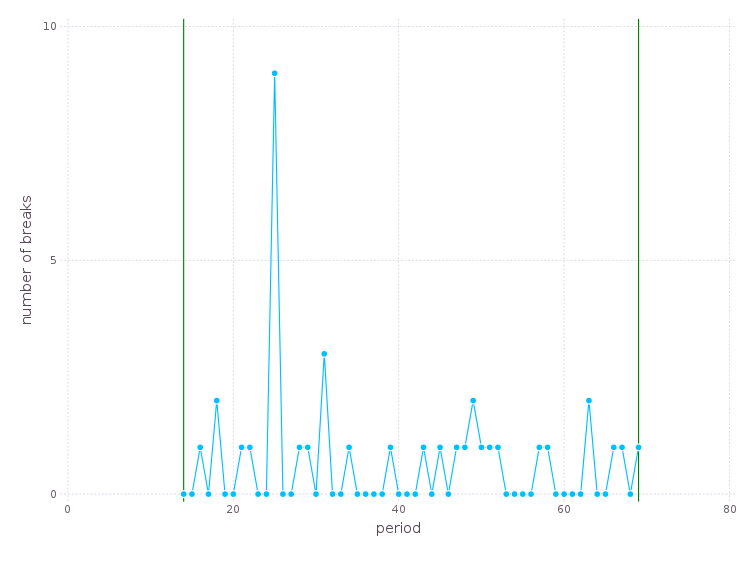
\includegraphics[width=8cm]{graphs/structural_breaks_less_variables.png}}
	\subfloat[1\% significance level]{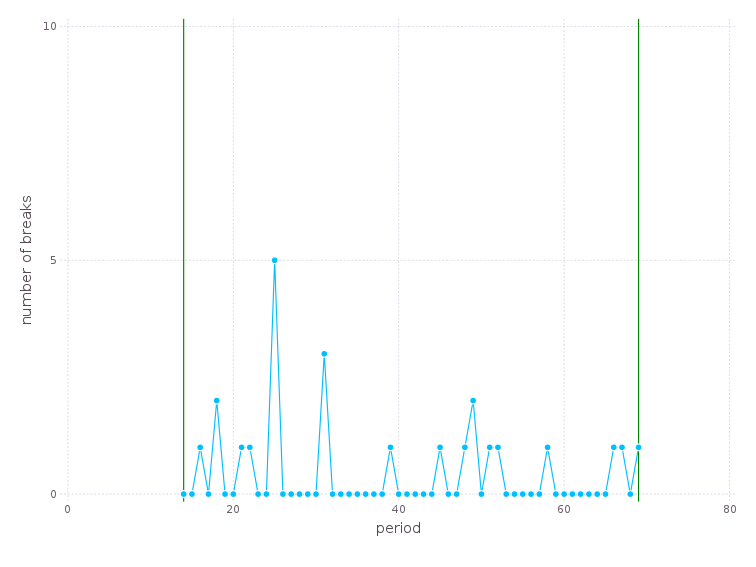
\includegraphics[width=8cm]{graphs/structural_breaks_less_variables_1percent.png}}
	\caption{Second cluster removed}
	\label{reduced data set, second cluster removed}
\end{figure}
	
\begin{figure}[htp]
	\subfloat[5\% significance level]{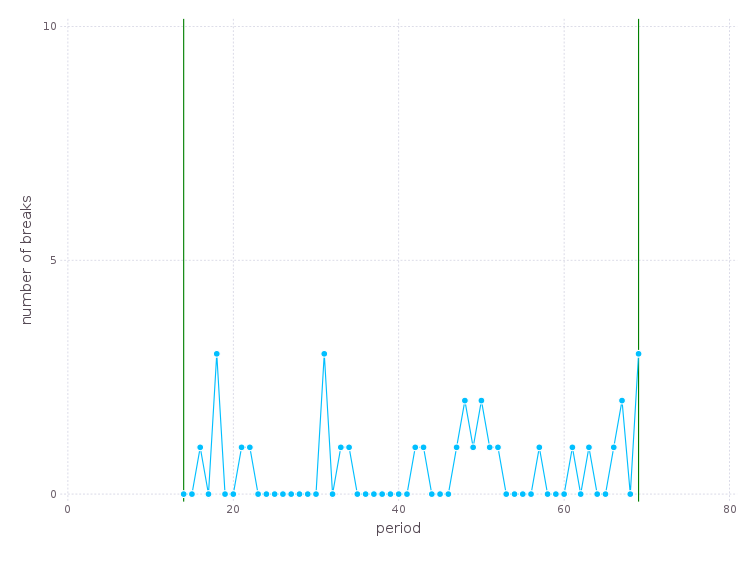
\includegraphics[width=8cm]{graphs/structural_breaks_even_less_variables.png}}
	\subfloat[1\% significance level]{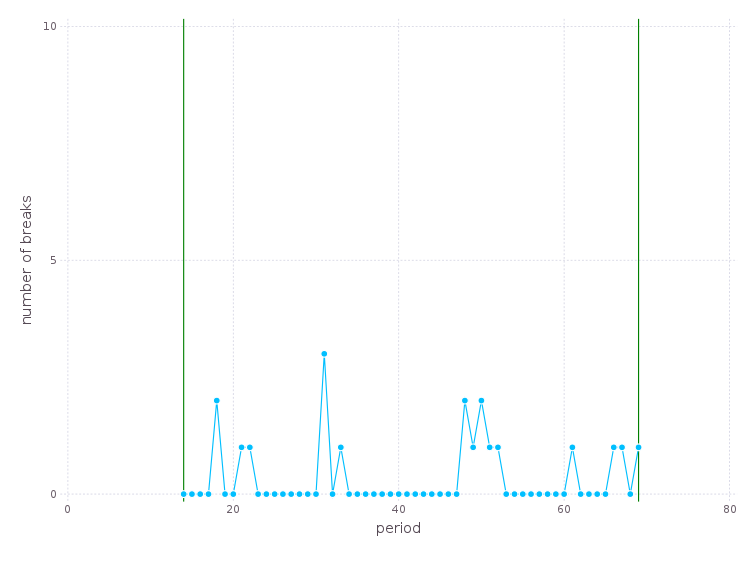
\includegraphics[width=8cm]{graphs/structural_breaks_even_less_variables_1percent.png}}
	\caption{First and second cluster removed}
	\label{reduced data set, first and second cluster removed}
\end{figure}

\begin{figure}[htp]
	\centering
	\subfloat[5\% significance level]{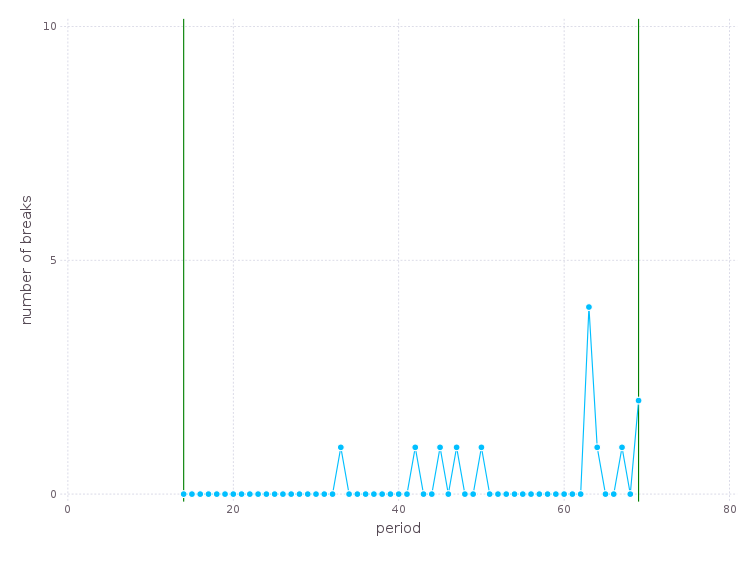
\includegraphics[width=8cm]{graphs/structural_breaks_all_breaks_removed.png}}
	\subfloat[1\% significance level]{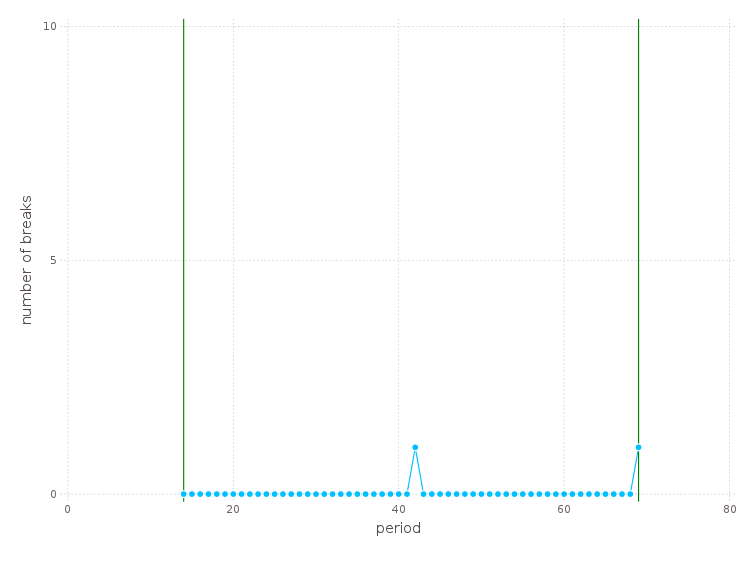
\includegraphics[width=8cm]{graphs/structural_breaks_all_breaks_removed_1percent.png}}
	\caption{All variables with breaks removed}
	\label{reduced data set, all variables with breaks removed}
\end{figure}

\begin{figure}[htp]
	\centering
	\subfloat[5\% significance level]{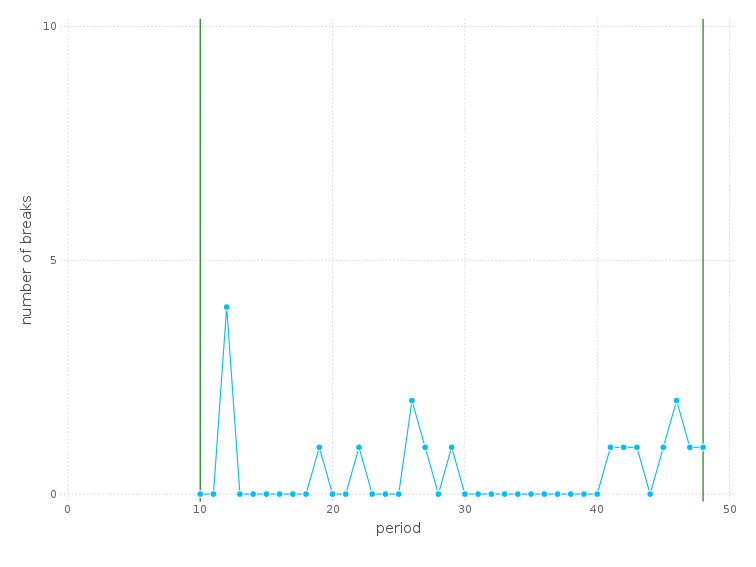
\includegraphics[width=8cm]{graphs/structural_breaks_second_cluster_and_obs_removed.png}}
	\subfloat[1\% significance level]{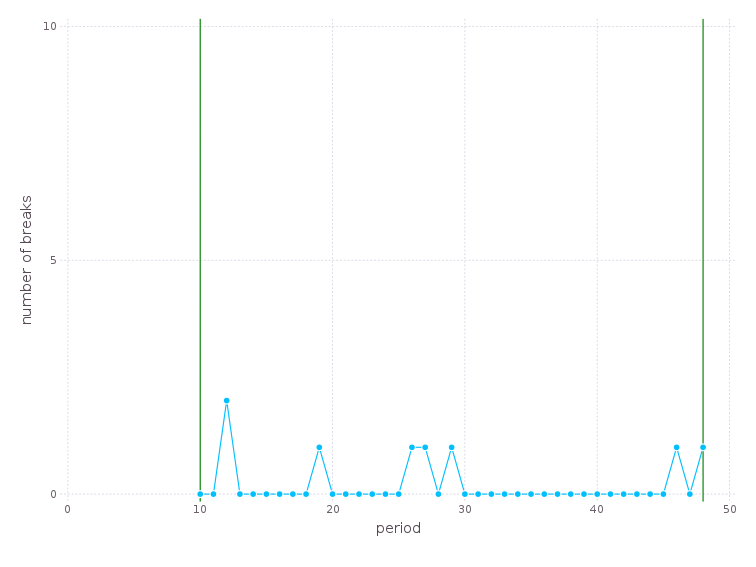
\includegraphics[width=8cm]{graphs/structural_breaks_second_cluster_and_obs_removed_1percent.png}}
	\caption{Second cluster removed, data set trimmed before 1991 quarter 1}
	\label{reduced data set, second cluster removed, data set trimmed}
\end{figure}



\clearpage
\newpage

\section{Interaction: Targeted predictors, removal of breaks}
\begin{table}[htp]
	\centering
	\begin{tabular}{cc|lll|lll}
		k & N$_{\text{breaks removed}}$ & RMSE$_{\text{tar}}$ & RMSE$_{\text{br}}$ & $\Delta_{\text{RMSE}}$ &  DM & $p_>$ & $p_{\not =}$ \\
		\hline
			26 & 18 & 0.4809 & 0.4564 & 0.0245 & 0.4965 & 0.3136 & 0.6272 \\
			27 & 19 & 0.4823 & 0.4602 & 0.0221 & -0.4547 & 0.6718 & 0.6563 \\
			28 & 18 & 0.4957 & 0.4528 & 0.0429 & -0.2979 & 0.6149 & 0.7701 \\
			29 & 18 & 0.4927 & 0.4806 & 0.0121 & 0.0883 & 0.4654 & 0.9309 \\
			30 & 17 & 0.4925 & 0.4959 & -0.0034 & 0.5863 & 0.2835 & 0.5670 \\
			31 & 18 & 0.4943 & 0.4999 & -0.0055 & -0.1871 & 0.5729 & 0.8543 \\
			32 & 21 & 0.4014 & 0.4139 & -0.0125 & -0.5408 & 0.7014 & 0.5971 \\
			33 & 21 & 0.4747 & 0.4295 & 0.0452 & -1.9228 & 0.9625 & 0.0751 \\
			34 & 22 & 0.4849 & 0.4501 & 0.0349 & -1.9577 & 0.9647 & 0.0705 \\
			35 & 24 & 0.4217 & 0.5230 & -0.1013 & -0.7701 & 0.7730 & 0.4541 \\
			36 & 24 & 0.4826 & 0.4620 & 0.0206 & -1.1949 & 0.8740 & 0.2520 \\
			37 & 25 & 0.4442 & 0.4530 & -0.0088 & -1.2802 & 0.8894 & 0.2213 \\
			38 & 26 & 0.4312 & 0.4785 & -0.0473 & -1.0385 & 0.8417 & 0.3167 \\
			39 & 27 & 0.4000 & 0.4811 & -0.0811 & -1.3551 & 0.9016 & 0.1968 \\
			40 & 28 & 0.4141 & 0.4856 & -0.0716 & -1.2543 & 0.8849 & 0.2303 \\
			41 & 27 & 0.4269 & 0.5076 & -0.0807 & -1.9239 & 0.9625 & 0.0749 \\
			42 & 28 & 0.4490 & 0.5048 & -0.0558 & -1.9349 & 0.9633 & 0.0735 \\
			43 & 28 & 0.4485 & 0.5084 & -0.0600 & -1.6533 & 0.9397 & 0.1205 \\
			44 & 29 & 0.4360 & 0.5192 & -0.0832 & -2.0236 & 0.9687 & 0.0625 \\
			45 & 30 & 0.4309 & 0.5237 & -0.0928 & -1.0432 & 0.8427 & 0.3145 \\
			46 & 31 & 0.4786 & 0.4948 & -0.0163 & -1.5163 & 0.9242 & 0.1517 \\
			47 & 32 & 0.4851 & 0.4943 & -0.0092 & -0.9166 & 0.8126 & 0.3748 \\
			48 & 33 & 0.4716 & 0.5000 & -0.0284 & -3.0493 & 0.9957 & 0.0087 \\ 
			49 & 33 & 0.5100 & 0.5000 & 0.0100 & 4.7581 & 0.0002 & 0.0003 \\
			50 & 35 & 0.5204 & 0.4579 & 0.0625 & -2.3135 & 0.9818 & 0.0364 \\ 
		\hline
	\end{tabular}
	\begin{minipage}{14cm}
		Critical values for the Diebold-Mariano test of improved and differing accuracy: \\ DM$_{1\%} = 2.62$, DM$_{5\%} = 1.76$, DM$_{10\%} = 1.35$ \\ DM$_{1\%} = 2.98$, DM$_{5\%} = 2.14$, DM$_{10\%} = 1.76$ (the relevant Statistic is $\text{abs}(\text{DM})$
	\end{minipage}
	\begin{minipage}{16cm}
		\small{\textbf{\textit{Notes:}} Entries report the performance of the optimal model achieved through targeting the predictors only (RMSE$_{\text{tar}}$) and removing the structural breaks from the targeted data sets afterwards (RMSE$_{\text{br}}$). The data sets have been targeted using soft thresholding with $k$ steps. N$_{\text{breaks removed}}$ is the number of variables left in the model after structural breaks are removed. DM denotes the small sample corrected Diebold Mariano statistic from \citet{harvey1997testing}. $p_>$ and $p_{\not =}$ denote the p-values of a test for improved and differing forecasting accuracy respectively.}
	\end{minipage}
	\caption{RMSE after removing structural breaks from targeted data}
	\label{diff rmse by removing breaks after targeting}
\end{table}





\clearpage
\newpage

\section{Data series}
\label{Data series}


\begin{table}[ht]
\caption{Federal Reserve Saint Louis data series}
\label{fred data}
\centering
\begin{tabular}{r|p{4cm}p{11cm}}
  \hline
  & Series ID & Series Description \\ 
  \hline
	1 & A229RX0 & Real Disposable Personal Income: Per capita \\ 
	\hline
	2 & AAA & Moody's Seasoned Aaa Corporate Bond Yield© \\ 
	\hline
	3 & ACNGNO & Value of Manufacturers' New Orders for Consumer Goods: Consumer Nondurable Goods Industries \\ 
	\hline
	4 & AHECONS & Average Hourly Earnings Of Production And Nonsupervisory Employees: Construction \\ 
	\hline
	5 & AHEMAN & Average Hourly Earnings Of Production And Nonsupervisory Employees: Manufacturing \\ 
	\hline
	  6 & AHETPI & Average Hourly Earnings of Production and Nonsupervisory Employees: Total Private \\ 
	\hline
	7 & AWHMAN & Average Weekly Hours of Production and Nonsupervisory Employees: Manufacturing \\ 
	\hline
	8 & AWOTMAN & Average Weekly Overtime Hours of Production and Nonsupervisory Employees: Manufacturing \\ 
	\hline
	9 & BAA & Moody's Seasoned Baa Corporate Bond Yield© \\ 
	\hline
    10 & BOGMBASE & Monetary Base; Total \\ 
    \hline
	11 & BOGNONBR & Non-Borrowed Reserves of Depository Institutions (DISCONTINUED SERIES) \\ 
	\hline
	12 & BUSLOANS & Commercial and Industrial Loans, All Commercial Banks \\ 
	\hline
	13 & BUSLOANSNSA & Commercial and Industrial Loans, All Commercial Banks \\ 
	\hline
	14 & CCRETT01USM661N & Real Effective Exchange Rates Based on Manufacturing Consumer Price Index for the United States© \\ 
	\hline
	15 & CES0600000007 & Average Weekly Hours of Production and Nonsupervisory Employees: Goods-Producing \\ 
	\hline

\end{tabular}
\end{table}

\begin{table}[ht]
\label{fred data 2}
\centering
\begin{tabular}{r|p{4cm}p{11cm}}
    \hline
	16 & CES0600000008 & Average Hourly Earnings of Production and Nonsupervisory Employees: Goods-Producing \\
	\hline
	17 & CES2000000008 & Average Hourly Earnings of Production and Nonsupervisory Employees: Construction \\ 
	\hline
	18 & CES3000000008 & Average Hourly Earnings of Production and Nonsupervisory Employees: Manufacturing \\ 	  \hline
	19 & CEU0500000008 & Average Hourly Earnings of Production and Nonsupervisory Employees: Total Private \\ 
	\hline
	20 & CEU0600000007 & Average Weekly Hours of Production and Nonsupervisory Employees: Goods-Producing \\ 
	\hline
	21 & CEU0600000008 & Average Hourly Earnings of Production and Nonsupervisory Employees: Goods-Producing \\ 
	\hline
	22 & CEU1000000001 & All Employees: Mining and Logging \\ 
	\hline
	23 & CEU2000000001 & All Employees: Construction \\ 
	\hline
	24 & CEU3000000001 & All Employees: Manufacturing \\ 
	\hline
	25 & CEU3000000007 & Average Weekly Hours of Production and Nonsupervisory Employees: Manufacturing \\ 
	\hline
	26 & CEU3000000009 & Average Weekly Overtime Hours of Production and Nonsupervisory Employees: Manufacturing \\ 
	\hline
	27 & CEU3100000001 & All Employees: Durable Goods \\ 
	\hline
	28 & CEU3200000001 & All Employees: Nondurable Goods \\ 
	\hline
	29 & CEU9000000001 & All Employees: Government \\ 
	\hline
	30 & CIVPART & Civilian Labor Force Participation Rate \\ 
	\hline
	31 & CLF16OV & Civilian Labor Force \\ 
	\hline
	32 & CPALTT01USM661S & Consumer Price Index: Total All Items for the United States© \\ 
	\hline
	33 & CPIAPPNS & Consumer Price Index for All Urban Consumers: Apparel \\ 
	\hline
	34 & CPIAPPSL & Consumer Price Index for All Urban Consumers: Apparel \\ 
	\hline
	35 & CPIAUCNS & Consumer Price Index for All Urban Consumers: All Items \\ 
	\hline
	36 & CPIAUCSL & Consumer Price Index for All Urban Consumers: All Items \\ 
	\hline
	37 & CPILFENS & Consumer Price Index for All Urban Consumers: All Items Less Food \& Energy \\ 
	\hline
	38 & CPILFESL & Consumer Price Index for All Urban Consumers: All Items Less Food \& Energy \\ 
	\hline
	39 & CPIMEDNS & Consumer Price Index for All Urban Consumers: Medical Care \\ 
	\hline
	40 & CPIMEDSL & Consumer Price Index for All Urban Consumers: Medical Care \\ 
	\hline
\end{tabular}
\end{table}

\begin{table}[ht]
\label{fred data 3}
\centering
\begin{tabular}{r|p{4cm}p{11cm}}
    \hline
	41 & CPITRNNS & Consumer Price Index for All Urban Consumers: Transportation \\ 
	\hline
	42 & CPITRNSL & Consumer Price Index for All Urban Consumers: Transportation \\ 
	\hline
	43 & CURRNS & Currency Component of M1 \\ 
	\hline
	44 & CURRSL & Currency Component of M1 \\ 
	\hline
	45 & DGORDER & Manufacturers' New Orders: Durable Goods \\ 
	\hline
	46 & DMANEMP & All Employees: Durable goods \\ 
	\hline
	47 & EXCAUS & Canada / U.S. Foreign Exchange Rate \\ 
	\hline
	48 & EXJPUS & Japan / U.S. Foreign Exchange Rate \\ 
	\hline
	49 & EXSZUS & Switzerland / U.S. Foreign Exchange Rate \\ 
	\hline
	50 & EXUSUK & U.S. / U.K. Foreign Exchange Rate \\ 
	\hline
	51 & FEDFUNDS & Effective Federal Funds Rate \\ 
	\hline
	52 & GS1 & 1-Year Treasury Constant Maturity Rate \\ 
	\hline
	53 & GS5 & 5-Year Treasury Constant Maturity Rate \\ 
	\hline
	54 & HOUST & Housing Starts: Total: New Privately Owned Housing Units Started \\ 
	\hline
	55 & HOUSTMW & Housing Starts in Midwest Census Region \\ 
	\hline
	56 & HOUSTMWNSA & Housing Starts in Midwest Census Region \\ 
	\hline
	57 & HOUSTNE & Housing Starts in Northeast Census Region \\ 
	\hline
	58 & HOUSTNSA & Housing Starts: Total: New Privately Owned Housing Units Started \\ 
	\hline
	59 & HOUSTS & Housing Starts in South Census Region \\ 
	\hline
	60 & HOUSTSNSA & Housing Starts in South Census Region \\ 
	\hline
	61 & HOUSTW & Housing Starts in West Census Region \\ 
	\hline
	62 & HOUSTWNSA & Housing Starts in West Census Region \\ 
	\hline
	63 & INDPRO & Industrial Production Index \\ 
	\hline
	64 & IPBUSEQ & Industrial Production: Business Equipment \\ 
	\hline
	65 & IPCONGD & Industrial Production: Consumer Goods \\ 
	\hline
\end{tabular}
\end{table}

\begin{table}[ht]
\label{fred data 4}
\centering
\begin{tabular}{r|p{4cm}p{11cm}}
	\hline
	66 & IPDCONGD & Industrial Production: Durable Consumer Goods \\ 
	\hline
	67 & IPDMAN & Industrial Production: Durable Manufacturing (NAICS) \\ 
	\hline
	68 & IPFINAL & Industrial Production: Final Products (Market Group) \\ 
	\hline
	69 & IPFUELN & Industrial Production: Fuels \\ 
	\hline
	70 & IPFUELS & Industrial Production: Fuels \\ 
	\hline
	71 & IPMAN & Industrial Production: Manufacturing (NAICS) \\ 
	\hline
	72 & IPMAT & Industrial Production: Materials \\ 
	\hline
	73 & IPMINE & Industrial Production: Mining \\ 
	\hline
	74 & IPNCONGD & Industrial Production: Nondurable Consumer Goods \\ 
	\hline
	75 & ISRATIO & Total Business: Inventories to Sales Ratio \\ 
	\hline
	76 & LNS12032197 & Employment Level - Part-Time for Economic Reasons, Nonagricultural Industries \\ 
	\hline
	77 & LNU01000000 & Civilian Labor Force \\ 
	\hline
	78 & LNU01300000 & Civilian Labor Force Participation Rate \\ 
	\hline
	79 & M1NS & M1 Money Stock \\ 
	\hline
	80 & M1SL & M1 Money Stock \\ 
	\hline
	81 & M2NS & M2 Money Stock \\ 
	\hline
	82 & M2SL & M2 Money Stock \\ 
	\hline
	83 & MABMM301USM189S & M3 for the United States© \\ 
	\hline
	84 & MANEMP & All Employees: Manufacturing \\ 
	\hline
	85 & MCUMFN & Capacity Utilization: Manufacturing (NAICS) \\ 
	\hline
	86 & MICH & University of Michigan Inflation Expectation© \\ 
	\hline
	87 & NAPM & ISM Manufacturing: PMI Composite Index© \\ 
	\hline
	88 & NAPMEI & ISM Manufacturing: Employment Index© \\ 
	\hline
	89 & NAPMII & ISM Manufacturing: Inventories Index© \\ 
	\hline
	90 & NAPMNOI & ISM Manufacturing: New Orders Index© \\ 
	\hline
\end{tabular}
\end{table}

\begin{table}[ht]
\label{fred data 5}
\centering
\begin{tabular}{r|p{4cm}p{11cm}}
	\hline	
	91 & NAPMPI & ISM Manufacturing: Production Index© \\ 
	\hline
	92 & NAPMSDI & ISM Manufacturing: Supplier Deliveries Index© \\ 
	\hline
	93 & NDMANEMP & All Employees: Nondurable goods \\ 
	\hline
	94 & NEWORDER & Manufacturers' New Orders: Nondefense Capital Goods Excluding Aircraft \\ 
	\hline
	95 & PAYEMS & All Employees: Total nonfarm \\ 
	\hline
	96 & PAYNSA & All Employees: Total nonfarm \\ 
	\hline
	97 & PERMITNSA & New Privately-Owned Housing Units Authorized by Building Permits: Total \\ 
	\hline
	98 & PPIACO & Producer Price Index: All Commodities \\ 
	\hline
	99 & PPICRM & Producer Price Index: Crude Materials for Further Processing \\ 
	\hline
	100 & PPIFCF & Producer Price Index: Finished Consumer Foods \\ 
	\hline
	101 & PPIFGS & Producer Price Index: Finished Goods \\ 
	\hline
	102 & PPIITM & Producer Price Index: Intermediate Materials: Supplies \& Components \\ 
	\hline
	103 & RRSFS & Real Retail and Food Services Sales \\ 
	\hline
	104 & SRVPRD & All Employees: Service-Providing Industries \\ 
	\hline
	105 & TB3MS & 3-Month Treasury Bill: Secondary Market Rate \\ 
	\hline
	106 & TB6MS & 6-Month Treasury Bill: Secondary Market Rate \\ 
	\hline
	107 & TCU & Capacity Utilization: Total Industry \\ 
	\hline
	108 & TOTBUSIMNSA & Total Business Inventories \\ 
	\hline
	109 & TOTBUSIRNSA & Total Business: Inventories to Sales Ratio \\ 
	\hline
	110 & UCNGNO & Value of Manufacturers' New Orders for Consumer Goods: Consumer Nondurable Goods Industries \\ 
	\hline
	111 & UEMPMEAN & Average (Mean) Duration of Unemployment \\ 
	\hline
	112 & UMCSENT & University of Michigan: Consumer Sentiment© \\ 
	\hline
	113 & UNEMPLOY & Unemployed \\ 
	\hline
	114 & UNRATE & Civilian Unemployment Rate \\ 
	\hline
	115 & UNRATENSA & Civilian Unemployment Rate \\ 
	\hline
	116 & USCONS & All Employees: Construction \\ 
	\hline
	117 & USGOOD & All Employees: Goods-Producing Industries \\ 
	\hline
	118 & USGOVT & All Employees: Government \\ 
	\hline
	119 & USMINE & All Employees: Mining and logging \\ 
	\hline
	120 & W875RX1 & Real personal income excluding current transfer receipts \\ 
	\hline
	\hline
\end{tabular}
\end{table}

\begin{table}[ht]
\caption{Bundesbank data series}
\label{bb data}
\centering
\begin{tabular}{r|p{4cm}p{11cm}}
	\hline
	& Series ID & Series Description \\
	\hline
	121 & BBK01. JQA000 & National accounts/Overall economic view/At current prices/ GDP \\ 
	\hline
	122 & BBDE1. M.DE.N. AEA1. A2P300000. F.C.I10.L & Orders received / At constant prices / Germany / Industry /
	 Unadjusted figure \\ 
	 \hline
	123 & BBDE1. M.DE.N. BAA1. P2XF00000. G.C.I10.L & Output in the production sector / At constant prices / Germany / Main construction industry / Unadjusted figure \\ 
	\hline
	124 & BBDE1. M.DE.W. AEA1. A2P310000. F.V.I10.A & Orders received / At current prices / Germany / Industry / Calendar adjusted only \\ 
	\hline
	125 & BBDE1. M.DE.W. AEA1. P2XF00000. B2.V.I10.A & Orders received / At current prices, flows / Germany / Main construction industry / Calendar adjusted only \\ 
	\hline
	126 & BBDE1. M.DE.Y. AEA1. A2P300000. F.V.I10.A & Orders received / At current prices / Germany / Industry / Calendar and seasonally adjusted \\ 
	\hline
	127 & BBDE1. M.DE.Y. AEA1. A2R200050. F.V.I10.A & Orders received / At current prices, flows / Germany / 20+21 Manufacture of chemicals, chemical products; basic pharmaceutical products and pharmaceutical preparations / Calendar and seasonally adjusted \\ 
	\hline
	128 & BBDE1. M.DE.Y. AEA1. P2XF00000. B2.C.I10.A & Orders received / At constant prices / Germany / Main construction industry / Calendar and seasonally adjusted \\ 
	\hline
	129 & BBDE1. M.DE.Y. AEA1. P2XF02000. B2.V.I10.A & Orders received / At current prices, flows / Germany / Main construction industry / Calendar and seasonally adjusted \\ 
	\hline
	130 & BBDE1. M.DE.Y. AEB1. A2P310000. F.V.I10.A & Orders received from the domestic market / At current prices / Germany / Industry / Calendar and seasonally adjusted \\ 
	\hline
\end{tabular}
\end{table}

\begin{table}[ht]
\centering
\begin{tabular}{r|p{4cm}p{11cm}}
	\hline
	131 & BBDE1. M.DE.Y. AEB1. N2C290000. F.C.I10.A & Orders received from the domestic market / At constant prices / Germany / 20+21 Manufacture of chemicals, chemical products; basic pharmaceutical products and pharmaceutical preparations / Calendar and seasonally adjusted \\ 
	\hline
	132 & BBDE1. M.DE.Y. AEB5. A2P300000. F.V.I10.A & Orders received from abroad / At current prices / Germany / Industry / Calendar and seasonally adjusted \\ 
	\hline
	133 & BBDE1. M.DE.Y. BA01. A2P200000. F.C.I10.A & Produktionsergebnis je Beschäftigten / Deutschland / Bergbau und Gewinnung von Steinen und Erden sowie Verarbeitendes Gewerbe (B + C) / Angaben für fachliche Betriebsteile / kalender- und saisonbereinigt \\ 
	\hline
	134 & BBDE1. M.DE.Y. BAA1. A2P000000. G.C.I10.A & Output in the production sector / Germany / Production sector including construction (B -F) / Calendar and seasonally adjusted \\ 
	\hline
	135 & BBDE1. M.DE.Y. BEA1. P2XF00000. BA.P.ABA.A & Employed persons (including proprietors and family workers) / Persons / Germany / Main construction industry / Calendar and seasonally adjusted \\ 
	\hline
	136 & BBDP1. M.DE.N. APA1.G. GP09SA000000. I10.A & Construction price index / Germany / Unadjusted figure / Total \\ 
	\hline
	137 & BBDP1. M.DE.N. VPI.C. A00000. I10.L & Consumer price index / Germany / Unadjusted figure / Total \\ 
	\hline
	138 & BBDP1. M.DE.Y. APA1.G. GP09SA000000. I10.A & Indices of foreign trade prices - exports, total / Germany / Calendar and seasonally adjusted / Total \\ 
	\hline
	139 & BBDP1. M.DE.Y. EPL.L. L1A00000000. I10.A & Index of producer prices of industrial products sold on the domestic market / Germany / Calendar and seasonally adjusted / Total \\ 
	\hline
	140 & BBEE1. M.DE.AAA. XY0B02. R.AACPB. M00 & Indicator of the German economy's price competitiveness against 24 selected industrial countries, based on the deflators of total sales \\ 
	\hline
	141 & BBEX3. M.XAU. USD.EA. AC.C06 & Price of gold in London / morning fixing * / 1 ounce of fine gold = USD ... \\
	\hline 
	142 & BBK01. BU1132 & Central government debt - total debt \\ 
	\hline
	143 & BBK01. DU7802 & Basic pay rates, overall economy, excluding ancillary benefits, excluding one-off
	 payments, on a monthly basis, Germany \\ 
	 \hline
	144 & BBK01. ES4710 & Balance on current account / Seasonally adjusted \\ 
	\hline
	145 & BBK01. EU2001 & Foreign trade / Exports (fob) \\ 
	\hline
\end{tabular}
\end{table}

\begin{table}[ht]
\centering
\begin{tabular}{r|p{4cm}p{11cm}}
	\hline
	146 & BBK01. EU4170 & Income / Total / Receipts \\ 
	\hline
	147 & BBK01. EU4670 & Financial transactions / Other investment / Balance \\ 
	\hline
	148 & BBK01. EU4680 & Foreign investment in Germany / Other investment / Total / Balance \\ 
	\hline
	149 & BBK01. OU0092 & Lending to domestic banks (MFIs) / Credit balances and loans / All categories of banks \\ 
	\hline
	150 & BBK01. OU0144 & Medium and long-term lending to general government / Loans / Medium-term / All categories of banks \\ 
	\hline
	151 & BBK01. OU0149 & Medium and long-term lending to general government / Loans / Long-term / All categories of banks \\ 
	\hline
	152 & BBK01. OU0337 & Medium and long-term lending / to general government / Securities / All categories of banks \\ 
	\hline
	153 & BBK01. OU0778 & Lending to banks (MFIs) / Total / All categories of banks \\ 
	\hline
	154 & BBK01. OU1429 & Lending to banks (MFIs) / Balances and loans / All categories of banks \\ 
	\hline
	155 & BBK01. OU1825 & Capital / Total / All categories of banks \\ 
	\hline
	156 & BBK01. TUD317 & MONEY STOCK M1 (FROM 2002, EXCLUDING CURRENCY IN CIRCULATION) / GERMAN CONTRIBUTION 
	\\ 
	\hline
	157 & BBK01. TVS303J & Geldmenge M1 /                                                   Veränderung saisonbereinigt / Jahresrate / EWU \\ 
	\hline
	158 & BBK01. TXI355 & TOTAL ASSETS OR LIABILITIES / GERMAN CONTRIBUTION \\ 
	\hline
	159 & BBK01. US02CC & Employees subject to social security contributions / Total / Western Germany / Seasonally adjusted / 1 / 2 \\ 
	\hline
	160 & BBK01. US0CC1 & Employees subject to social security contributions / Total / Eastern Germany / Seasonally adjusted / 1 / 2 \\ 
	\hline
	161 & BBK01. USBA14 & Employment in Germany / Employed persons in Germany / Germany / Seasonally adjusted / 1 / 2 \\ 
	\hline
	162 & BBK01. UUCY01 & Unemployment rate (unemployment as a percentage of the civilian labour force) / Germany / 1 / 2 / 3 \\ 
	\hline
	163 & BBK01. WU0028 & Gross sales of domestic debt securities at nominal value / Total \\ 
	\hline
	164 & BBK01. WU3141 & DAX price index / End 1987 = 1000 / End of month \\ 
	\hline
	165 & BBK01. XS7085 & Exports / European countries / Seasonally adjusted \\ 
	\hline
	166 & BBK01. XU4204 & German exports / special trade / values / 1 / 2 / 3 / 4 \\ 
	\hline
	167 & BBK01. XU4205 & German imports / special trade / values / 1 / 2 / 3 / 4 \\ 
	\hline
	168 & BBK01. XU4206 & German foreign trade balance / special trade / values / 1 / 2 / 3 / 4 \\ 
	\hline
	169 & BBK01. XX3739 & Exports of the Federal Republic of Germany / Special Trade / Total / 1 / 2 / \\ 
	\hline
    \hline
\end{tabular}
\end{table}


\clearpage
\newpage
\section{Replication and data files}
\label{replication and data files}
All replication files can be found at \url{https://github.com/joidegn/Masterarbeit} or can be gotten from the author by request.

A result from writing this thesis is the FactorModels Julia package which has been released in the public domain as free software licensed under the MIT License a copy of which can be found at \url{http://opensource.org/licenses/MIT}. Julia, is a powerful, open-source technical computing language which can be found at \url{http://julialang.org/}. The FactorModels package does the heavy lifting for the replication files and has to be installed in order to run them. Instructions on how to replicate the results are provided both with the package and the replication files.


\clearpage
\newpage
\bibliographystyle{plainnat}
\bibliography{/home/joi/workspace/latex/citations}

\clearpage
\newpage
\addcontentsline{toc}{section}{Statutory Declaration}
\restoregeometry
\thispagestyle{empty}
\singlespacing



\centering{\section*{Declaration}}
\raggedright
\begin{enumerate}
\item{I hereby declare that this thesis, entitled: \\
\vspace{0.5cm}
\begin{center}
	\textbf{Predicting Economic Time-Series using Dynamic Factor Models under Structural Breaks}
\end{center}

%\underline{\hspace{15cm}} \\
%\underline{\hspace{15cm}} \\
%\underline{\hspace{15cm}} \\

is a result of my own work and that no other than the indicated aids have been used for
its completion. Material borrowed directly or indirectly from the works of others is
indicated in each individual case by acknowledgement of the source and also the
secondary literature used.
This work has not previously been submitted to any other examining authority and has
not yet been published.
}

\item{After completion of the examining process, this work will be given to the library of the
University of Konstanz, where it will be accessible to the public for viewing and borrowing. As author of this work, I agree to this procedure.}
\end{enumerate}

\vspace{1cm}
Konstanz, \underline{\hspace{4cm}} \hspace{3cm} \underline{\hspace{6cm}}
\\
\vspace{1cm}

\centering{\section*{Erklärung}}
\raggedright
\begin{enumerate}
\item{ Ich versichere hiermit, dass ich die vorliegende Arbeit mit dem Thema: \\
\vspace{0.5cm}
\begin{center}
	\textbf{Predicting Economic Time-Series using Dynamic Factor Models under Structural Breaks}
\end{center}

selbständig verfasst und keine anderen Hilfsmittel als die angegebenen benutzt habe.
Die Stellen, die anderen Werken dem Wortlaut oder dem Sinne nach entnommen sind,
habe ich in jedem einzelnen Falle durch Angaben der Quelle, auch der benutzten
Sekundärliteratur, als Entlehnung kenntlich gemacht. Die Arbeit wurde bisher keiner
anderen Prüfungsbehörde vorgelegt und auch noch nicht veröffentlicht.}

\item{Diese Arbeit wird nach Abschluss des Prüfungsverfahrens der Universitätsbibliothek
Konstanz übergeben und ist durch Einsicht und Ausleihe somit der Öffentlichkeit
zugänglich. Als Urheber der anliegenden Arbeit stimme ich diesem Verfahren zu.}
\end{enumerate}

\vspace{1cm}
Konstanz, den \underline{\hspace{3.3cm}} \hspace{3cm} \underline{\hspace{6cm}}

\end{document}
